%%%%%%%% Thesis: Where Confidence Gets Laundered (long form, 2026-10-07) %%%%%%%%
% Every number in this document is copied from docs/paper/main.tex (v5, 2026-09-25)
% or from a json under analysis/cloud/ (nested_3.7b.json, shortcut_k2-3.7b.json,
% cascade/curves.json, verbal/audit.json). Tables in Part II are the paper's
% tables, copied verbatim. Planning quantities in Part IV (the $500 allowance, the
% per-run dollar quotes) come from goal/GOAL.md, docs/goal-2026-09-21.md and
% docs/design-*.md and are marked as plans; no hour count is stated anywhere.
% Three tags run through the text: [SHOWN] = measured, with a control, in
% main.tex or analysis/cloud; [SUGGESTED] = direction consistent, interval
% includes zero; [BET] = no evidence yet, a dated prediction or a plan.
% Build: cd docs/thesis && PATH=/Library/TeX/texbin:$PATH latexmk -pdf thesis.tex && latexmk -c

\documentclass[11pt,a4paper]{report}

\usepackage[margin=2.1cm,marginparwidth=1.6cm,marginparsep=0.25cm]{geometry}
\usepackage{etoolbox}
\usepackage{titlesec}
\usepackage[hyphens]{url}
\usepackage{microtype}
\usepackage{booktabs}
\usepackage{graphicx}
\graphicspath{{../paper/figs/}}
\usepackage{amsmath}
\usepackage{amssymb}
\usepackage{mathtools}
\usepackage{xcolor}
\usepackage{multirow}
\usepackage{subcaption}
\usepackage{enumitem}
\usepackage{marginnote}
\usepackage{pgfplots}
\pgfplotsset{compat=1.18}
\usepackage[most]{tcolorbox}
\usepackage{natbib}
\usepackage[colorlinks=true,linkcolor=blue!50!black,citecolor=blue!50!black,urlcolor=blue!50!black]{hyperref}
\usepackage[capitalize,noabbrev]{cleveref}

\setlist{itemsep=2pt,topsep=3pt}
\setlength{\parskip}{2pt}
\emergencystretch=1.5em

% ---- status tags -----------------------------------------------------------
\definecolor{shownc}{RGB}{0,110,40}
\definecolor{suggc}{RGB}{185,110,0}
\definecolor{betc}{RGB}{160,20,20}
\newcommand{\SHOWN}{\textcolor{shownc}{\textbf{\scriptsize[SHOWN]}}}
\newcommand{\SUGG}{\textcolor{suggc}{\textbf{\scriptsize[SUGGESTED]}}}
\newcommand{\BET}{\textcolor{betc}{\textbf{\scriptsize[BET]}}}
\newcommand{\mshown}{\marginnote{\SHOWN}}
\newcommand{\msugg}{\marginnote{\SUGG}}
\newcommand{\mbet}{\marginnote{\BET}}
\DeclareUrlCommand\src{\urlstyle{tt}}
\renewcommand{\UrlFont}{\footnotesize\ttfamily}
% chapters and parts continue on the current page (the document is long enough)
\makeatletter
\patchcmd{\chapter}{\if@openright\cleardoublepage\else\clearpage\fi}{\par\vspace{1.2em}}{}{}
\patchcmd{\part}{\if@openright\cleardoublepage\else\clearpage\fi}{\par\vspace{1.5em}}{}{}
\renewcommand\@endpart{\par\vspace{1.5em}}
\makeatother
\titleformat{\chapter}[hang]{\LARGE\bfseries}{\thechapter.}{0.6em}{}
\titlespacing*{\chapter}{0pt}{14pt}{12pt}
\titleclass{\part}{straight}
\titleformat{\part}[display]{\centering\Large\bfseries}{\partname~\thepart}{0.4em}{\huge}
\titlespacing*{\part}{0pt}{10pt}{20pt}
\setcounter{tocdepth}{1}

\crefname{part}{Part}{Parts}
\Crefname{part}{Part}{Parts}

\title{\textbf{Where Confidence Gets Laundered}\\[6pt]
\large The Label Carries the Signal, This Reader Discards It\\[10pt]
\normalsize A thesis on state handoffs between frozen language models:\\
what crossed, what did not, and what an economy of state would need}
\author{Peter\\ K2 Cascade project}
\date{2026-10-07 \quad (paper v5 numbers; no new runs)}

\begin{document}

\maketitle

\begin{abstract}
\noindent
A confidence word scored directly as a label predicts the sender's semantic entropy at AUROC .955 on clean passages; the receiver that reads that word lands at .552, within .02 of a receiver given no message at all (.532). The signal was in the message; this reader threw it away. \citet{2606.20662} had named the loss \emph{confidence laundering} and placed it in the text channel; the measurement here, 377 SQuAD items between a frozen K2-Horizon-3.7B sender and a frozen 7B receiver that is a base model under one completion prompt, places it at the reader. A mapped KV cache, which carries no label at all, leaves the receiver at .585 on the same items, nearly where reading the passage itself leaves it (.597), and moves the receiver's confidence within an item because of the cache's content (Spearman .280 against .004 for another item's cache). The cache is a real channel: 63.0\% on an 8-name binding test with chance at 12.5\%, the wrong episode's cache followed 63.7\% of the time, and 53.0 SQuAD F1 against 54.7 for text. It is also 72\,MiB per 512-token message. The second half of the document is a three-year program, one kill criterion per chapter. The reusable contribution is the audit: score the message, then the reader. Any paper that reports a verbal-confidence baseline should report the label-only AUROC next to the receiver AUROC.
\end{abstract}

\tableofcontents

\chapter*{What this document claims}
\addcontentsline{toc}{chapter}{What this document claims}

Three lists. A claim appears in exactly one of them. The tag that marks it here is the tag that marks it wherever it recurs in the text. SHOWN means a measurement with a control, reported in \src{docs/paper/main.tex} or in a json under \src{analysis/cloud/}. SUGGESTED means the direction is consistent across variants or seeds but at least one interval includes zero. BET means there is no evidence yet: a dated prediction from \src{docs/agent-communication-futures-2026-09-21.md} or \src{goal/GOAL.md}, or a plan in \cref{part:program}.

\begin{tcolorbox}[enhanced,breakable,colback=shownc!4,colframe=shownc,boxrule=0.6pt,arc=1pt,title={\textbf{SHOWN} (number, then control)}]
\small
\begin{itemize}[leftmargin=1.2em]
\item \textbf{The label carries the signal; this reader discards it.} Confidence word scored as a label: AUROC .955 / .942 / 1.000 (clean / contradicted / removed) against the sender's semantic entropy; the same word read by the receiver: .552 / .542 / .592. Control: the deranged cache at .536 / .488 / .564 and question-only at .532 / .479 / .603 bound what ``no message'' gives (\cref{ch:uncertainty,ch:where}).
\item \textbf{Content crosses.} 8-name binding test, $n = 1000$: trained projector 63.0\%, chance 12.5\%. Controls: the wrong episode's cache 4.6\% with the wrong value followed 63.7\% of the time; a projector trained with a deranged sender 23.4\% (ridge base 21.7\%); raw injection 14\% (\cref{ch:content}).
\item \textbf{Content crosses on real passages.} SQuAD F1 53.0 for the mapped cache against 54.7 for text and 16.6 for the question alone. Controls: wrong passage's cache 13.8, ridge 14.3, deranged-sender projector 15.1 (\cref{ch:passages}).
\item \textbf{The receiver's confidence moves because of the cache's content.} Within-item Spearman between receiver entropy change and sender SE change (clean $\to$ removed): cache .280, text .322, word .146. Control: another item's cache .004, which shares the question (\cref{ch:where}).
\item \textbf{Cache beats the word on contradicted passages.} Cache $-$ word $= [.008, .117]$, paired passage-grouped bootstrap; cache $-$ question-only $= [.065, .180]$ on the same variant (\cref{ch:uncertainty}).
\item \textbf{Text beats the cache on removed passages.} Cache $-$ text $= [-.091, -.002]$ (\cref{ch:uncertainty}).
\item \textbf{The recipe crosses one family boundary and fails on one pair.} Qwen3-4B $\to$ K2-7B: 71.7 $\pm$ 4.5\% over three seeds; K2-0.9B $\to$ 7B: 17.0\% (deranged 14.0\%) (\cref{ch:pairs}).
\item \textbf{The sender's state predicts its own failure.} Probe on the 3.7B's hidden state: AUROC .749 on 600 SQuAD items against its own semantic entropy at .689; .876 $[.813, .944]$ at layer 18 on 127 agent steps against trajectory metadata at .704 (\cref{ch:failed}, \src{analysis/cloud/cascade/curves.json}, \src{nested_3.7b.json}).
\item \textbf{Retention cannot tell a channel from a prompt.} The deranged-sender projector retains 0.77 of the continuation-loss gap, 0.72 of it with its input swapped; the binding test puts it near chance (\cref{ch:content}).
\item \textbf{The message costs 144\,KB per token}, 72\,MiB per 512-token prefix, about 604\,ms on a 1\,Gbps link against 24\,ms of receiver compute saved; int4 keeps 75.0\% / 51.6 F1 at 36\,KB per token; dropping layers collapses even under a filler null (\cref{ch:cost}).
\item \textbf{On SQuAD a handoff buys 3.5 F1 for 48\,ms per item, and the cache arm buys nothing.} Probe-triggered text handoff at rate 1: F1 52.2 $\to$ 55.7, latency 45 $\to$ 93\,ms per item; the cache handoff stays at 51.8. The kill written in \src{docs/design-cascade-2026-09-24.md} (state never beats text at equal cost) was met (\cref{ch:failed}, \src{analysis/cloud/cascade/curves.json}). Whether 3.5 F1 is worth 48\,ms is a price judgement, made in \cref{ch:program}, not a measurement.
\end{itemize}
\end{tcolorbox}

\begin{tcolorbox}[enhanced,breakable,colback=suggc!5,colframe=suggc,boxrule=0.6pt,arc=1pt,title={\textbf{SUGGESTED} (direction consistent, an interval includes zero)}]
\small
\begin{itemize}[leftmargin=1.2em]
\item The ordering text $\gtrsim$ cache $>$ word holds on all three variants (.597 / .615 / .671 vs .585 / .605 / .624 vs .552 / .542 / .592), but cache $-$ word includes zero on clean ($[-.027, .094]$) and removed ($[-.024, .086]$), and cache $-$ text includes zero on clean and contradicted.
\item The cache keeps more of the sender's confidence drop than the word (drop ratio .54 vs .30), a relative drop in $P(\text{gold})$ with no interval.
\item The receiver recovers the sender's alternatives about as well from the cache as from the passage (belief-shape Spearman .199 vs .193 on clean passages; controls .052 / .042); no interval, and the arms are not separated from each other.
\item Where the cache arm loses what it loses is not localised: sender state .739 / .706, one-position probe of the message .557 / .579, receiver via cache .643 / .563, via text .650 / .654.
\item Two receiver-side training objectives did not move the loss (drop ratio .56 and .51 against .54), which points at the sender side, without yet testing it.
\end{itemize}
\end{tcolorbox}

\begin{tcolorbox}[enhanced,breakable,colback=betc!4,colframe=betc,boxrule=0.6pt,arc=1pt,title={\textbf{BET} (no evidence yet; each carries a date or a kill criterion)}]
\small
\begin{itemize}[leftmargin=1.2em]
\item The unit of computation is becoming a population of models, and its protocol will move from text to state (\src{goal/GOAL.md}, north star sentences 1--2; no date, re-worded only).
\item A self-improving system will be a population handing state to each other and learning from what comes back (north star sentence 4, marked a bet there too).
\item A sender-side adapter trained on returned state raises the sender more than returned text at equal tokens (\cref{ch:p-return}; kill: (b) $-$ (a) $\le 0$ on three seeds).
\item On a task with a sender--receiver gap large enough to pay for a handoff, state beats text at equal measured cost only intra-GPU (\cref{ch:p-loop}; price sheet declared before the run).
\item A receiver-side detector tells a genuine mapped cache from a tampered one at AUROC $> .7$ (\cref{ch:p-fraud}).
\item From the futures document, three dated predictions this program can score: (11) a within-family KV projector loses more than 10 points of retention after a post-training update to the receiver, by 2027-12-31; (8) no replicated same-model multi-agent gain over 5 points at matched tokens with no private information, by 2028-12-31; (3) no production system passes latent state between two vendors across an organisational boundary, by 2030-12-31.
\item Latent state stays inside a shared-weights boundary for legal rather than technical reasons; if so, the population this thesis studies is one owner's models (\cref{ch:economy}).
\end{itemize}
\end{tcolorbox}

\paragraph{The handle.} One pair of numbers runs through the document: \textbf{.552 against .532}. The first is the receiver's AUROC against the sender's semantic entropy after it has read the confidence word on clean passages; the second is the same receiver given the question and no message. The receiver handed the label does no better than the receiver handed nothing, within .02 on clean, .063 on contradicted and $-.011$ on removed passages. The word's own score as a label, .955, enters only to establish that the message was not capacity-limited: it is a property of the label's construction (\cref{ch:where}), and the gap of .40 between the two is derived from it, not measured on its own. Everything else is context for that pair.

%=====================================================================
\part{The problem and the bet}
\label{part:problem}
%=====================================================================

\noindent The claim is that text launders confidence. It does not; this reader does.

\chapter{A population of models, and the claim they launder confidence}
\label{ch:population}

\section{The field's standing belief, in its own words}

\citet{2606.20662} titled their position paper \emph{Confidence Laundering in Agent Systems: Why Uncertainty Needs a Latent Carrier}. The claim is in the title. When a small model hands its answer to a larger one as text, with a word such as ``confidence: low'' attached, the larger model reads the answer and not the word; the hedge is washed out and a guess arrives downstream looking like a fact. Their remedy is in the title too: carry uncertainty in a latent, not in a sentence. They supported it with one experiment, Qwen-1.5B in a HotpotQA tool loop, a semantic-entropy label from 20 samples (as reported in \src{docs/lit-confidence-transfer-2026-09-22.md}, unverified against the PDF), and four handoffs scored by how well a downstream component ranks the high-entropy cases: answer only, answer plus a score, answer plus a textual description of uncertainty, answer plus a latent carrier. The latent carrier won. Their motivating picture is an edge--cloud stack that escalates from a small on-device model to a large one.

\section{The crack}

A low receiver-side score through a text handoff has two causes, and no handoff study had separated them.

Either the message does not carry the sender's uncertainty, or the reader does not use it. The first is a statement about a channel; the second is a statement about one model under one prompt. They call for different remedies, they generalise differently, and they cost one line of code to tell apart: score the message itself against the same target the receiver is scored against. If the message scores high and the receiver scores low, the loss is at the reader. If both score low, the loss is in the message. \citet{2606.20662} report the receiver's number only, with no content-free control, so their result is consistent with both readings. So is every text-versus-latent comparison we found through 2026-09-23 (\cref{app:reviews}).

This thesis is that one line, run properly: four kinds of handoff between the same two frozen models on the same items, with four content-free controls per passage variant, and the message scored before the reader on both label arms, the word and the number. The candidate-list arm, a full distribution, is not scored at message level; its entropy against the sender target would be near 1 by construction, as the word's is, and \cref{tab:tworows} says so rather than printing it.

\section{The two protocols side by side}

\Cref{tab:protocols} puts the position paper's measurement next to ours. The target is the same, AUROC against the sender's semantic entropy. The difference is in what sits around it.

\begin{table}[h]
\caption{The measurement of \citet{2606.20662} and the measurement in this thesis. Their column is taken from the description in \texttt{docs/paper/main.tex}, Related Work, except the two cells marked $\dagger$, which come from \texttt{docs/lit-confidence-transfer-2026-09-22.md} and carry that note's ``unverified'' flag (not checked against the PDF); ours from \texttt{main.tex}, Sections 2--5.}
\label{tab:protocols}
\vskip 0.1in
\centering
\small
\begin{tabular}{p{2.9cm}p{5.1cm}p{6.1cm}}
\toprule
 & Confidence Laundering (2606.20662) & This thesis \\
\midrule
target & sender semantic entropy, 20 samples, binarised$^\dagger$ & sender semantic entropy, 10 samples, median per variant \\
sender $\to$ receiver & Qwen-1.5B; downstream probe at blocks 7 / 14 / 28 & K2-Horizon-3.7B $\to$ K2-Horizon-7B, both frozen \\
handoffs & answer; $+$score; $+$textual uncertainty; $+$latent carrier & passage as text; answer $+$ word; $+$ number; $+$ candidate list; mapped KV cache \\
items & one HotpotQA tool loop; $N$ not stated$^\dagger$ & 377 SQuAD items $\times$ 3 passage variants (clean, contradicted, removed) \\
content-free controls & none & deranged cache, zero cache, moment-matched random cache, question only, per variant \\
intervals & none reported & paired, passage-grouped bootstrap on three cache differences \\
message scored directly & no & yes: label-only AUROC for the word and the number; linear probe for the cache \\
common-cause control & no & within-item intervention: question fixed, sender's passage changed \\
\bottomrule
\end{tabular}
\end{table}

The table is not a complaint about a position paper. It is the reason the thesis exists: the field's standing belief was stated with a measurement that could not distinguish its two readings. This document is the measurement that can, for any handoff whose message carries a label; for a state message, the carrier the position paper endorsed, it bounds what one position of the message carries and localises nothing yet (\cref{ch:where}). The stronger sentence holds for the word arm only.

\section{What the measurement found, in one paragraph}

On clean passages the receiver that reads the confidence word reaches AUROC .552 against the sender's semantic entropy; the receiver given no message reaches .532; the word scored directly as a label reaches .955 (SHOWN item 1). The signal was in the message. The reader, a base model under one completion prompt with no instruction to hedge, did not turn it into its own spread. That is what laundering looks like from inside, and it is a property of a reader, not of text. A mapped KV cache with no label at all leaves the receiver above both, and when the sender's passage is changed with the question held fixed the receiver's entropy moves with the sender's through the cache and not through another item's cache (SHOWN item 4). The cache carries something the receiver uses. What it carries is, by the parsimonious reading, the evidence; the receiver recomputes its own uncertainty from it, and no probe in this document isolates the sender's spread crossing as such. \SUGG\ \textbf{The label carries the signal, the reader discards it; the cache carries the evidence, the reader recomputes.}

\section{Contributions}

Three findings, each with the chapter that defends it.

\textbf{First}, the receiver-level ordering text $\gtrsim$ cache $>$ word, measured for four handoffs on 377 items with content-free controls per variant and paired passage-grouped intervals on the three cache differences, with cache $-$ word excluding zero on one variant of three (SHOWN item 5, SUGGESTED item 1) and the within-item intervention ruling out the question as a common cause (SHOWN item 4; \cref{ch:uncertainty,ch:where}).

\textbf{Second}, the \textbf{label-only audit} and the \textbf{two-level report} it belongs to: a message-level signal (the message scored against the sender target) next to a receiver-level signal (the receiver scored against the same target), with their difference the \textbf{read-out gap}. Applied here it relocates the text arm's loss from channel capacity to read-out for this receiver (SHOWN item 1; \cref{ch:where}). This is the reusable artefact of the thesis.

\textbf{Third}, the instrument's calibration: a channel whose content the receiver demonstrably reads, on a binding test and on real passages, that crosses one family boundary and fails on one pair, and whose bytes are counted (SHOWN items 2, 3, 7 and 10; \cref{ch:content,ch:pairs,ch:passages,ch:cost}).

The names are used from here without re-explanation. \emph{Message-level signal}, \emph{receiver-level signal}, \emph{read-out gap}, \emph{label-only audit}. When ``the audit'' appears alone it means the label-only audit: score the confidence label directly against the sender target, then score the receiver that read it.

%---------------------------------------------------------------------
\chapter{Text by inertia, and what state could carry}
\label{ch:state}

\section{Why the unit of computation is becoming a population}

A single model answering a single prompt is no longer the thing that gets deployed. Routers, cascades, speculative decoding and tool-calling agents are populations of models, and their protocol is text by inertia: it is what the models were trained to read, what humans can inspect, what logs can keep, and none of those is a reason it should be the protocol between two models that share nothing with a human reader. \BET\ This thesis bets the protocol moves to state (\src{goal/GOAL.md}, north star sentences 1--2), and measures the one piece of that bet two frozen models can settle: what a state handoff carries that a text handoff does not, against controls.

\section{Three things text cannot carry}

\src{goal/GOAL.md} names three: the computation already done, the shape of a belief (which alternatives, with what weight), and intermediate representations that are not words. Of the three, this thesis has measured the first and tried to measure the second.

\emph{The computation already done} is what the binding test and the SQuAD run measure. When the sender has read a passage and the receiver reads only the question, the receiver answers at 53.0 F1 through the mapped cache against 16.6 from the question alone. \SHOWN\ The sender's reading crossed. On an A100 the receiver would have spent 48\,ms re-reading 512 tokens; the projector takes 24\,ms. \SHOWN\ That is the saving, and \cref{ch:cost} says what it costs in bytes.

\emph{The shape of a belief} is what the uncertainty protocol tries to measure, and the result is that the receiver's confidence tracks the sender's through the cache about as well as through the passage itself, which is consistent with the evidence crossing and the receiver recomputing, and no experiment here isolates the shape crossing as such. \SUGG\ \Cref{ch:where} reports the diagnostic closest to the shape, the correlation between the sender's candidate frequencies and the receiver's first-token mass on those candidates, and it separates the arms from the controls, not from each other.

\emph{Intermediate representations that are not words} are not measured here at all. The setting is context reuse, the sender's cache of a passage prefix, not a mid-task handoff of an agent's reasoning or tool state, and nothing in this document says whether anything survives a sender that has reasoned at length \citep{2608.20927}. \BET\ \Cref{ch:p-loop} says what it would take to measure it.

\section{The read-out gap, named, with a toy example}
\label{sec:readout}

Fix a sender target $u_S$: a binary label, here ``the sender's semantic entropy is above its median.'' Fix a message $m$ that the sender produces. Score two things against $u_S$ with the same statistic, AUROC.

\begin{enumerate}
\item The \textbf{message-level signal}: the AUROC of a fixed function of $m$ alone. For a confidence word it is the rank of the word (low $>$ medium $>$ high). For a number it is the number. For a cache, which has no label, it is a linear probe on the mapped message, named as such wherever one appears.
\item The \textbf{receiver-level signal}: the AUROC of the receiver's first-token entropy after it has read $m$.
\end{enumerate}

Their difference is the \textbf{read-out gap}. It is a difference of two AUROCs, not an information decomposition; the cache's two levels use different instruments, so the gap is comparable within an arm and not across arms.

The toy example needs no numbers beyond definitions. Take a sender whose label is a perfect function of $u_S$ (the label says ``low'' exactly when $u_S = 1$). Its message-level AUROC is 1 by construction. Now take two readers. Reader A copies the label into its own entropy: high entropy when the label says low. Its receiver-level AUROC is also 1, and the read-out gap is 0. Reader B ignores the label and answers from its own knowledge of the question. Its entropy is independent of the label, its receiver-level AUROC is .5 (the definition of chance for the statistic), and the read-out gap is .5. Both readers received the same message. A study that reports only the receiver-level number would say that the text handoff ``laundered'' the sender's uncertainty for reader B, and would be unable to say whether the message or the reader was at fault. The audit says which: the message scored 1.

The measured version is \cref{fig:handle}. The label here is not perfect, because it is built from terciles over 587 items and scored against a median over the 377 kept items, but it is close: .955 / .942 / 1.000. The reader lands at .552 / .542 / .592. This reader is reader B.

\begin{figure}[h]
\centering
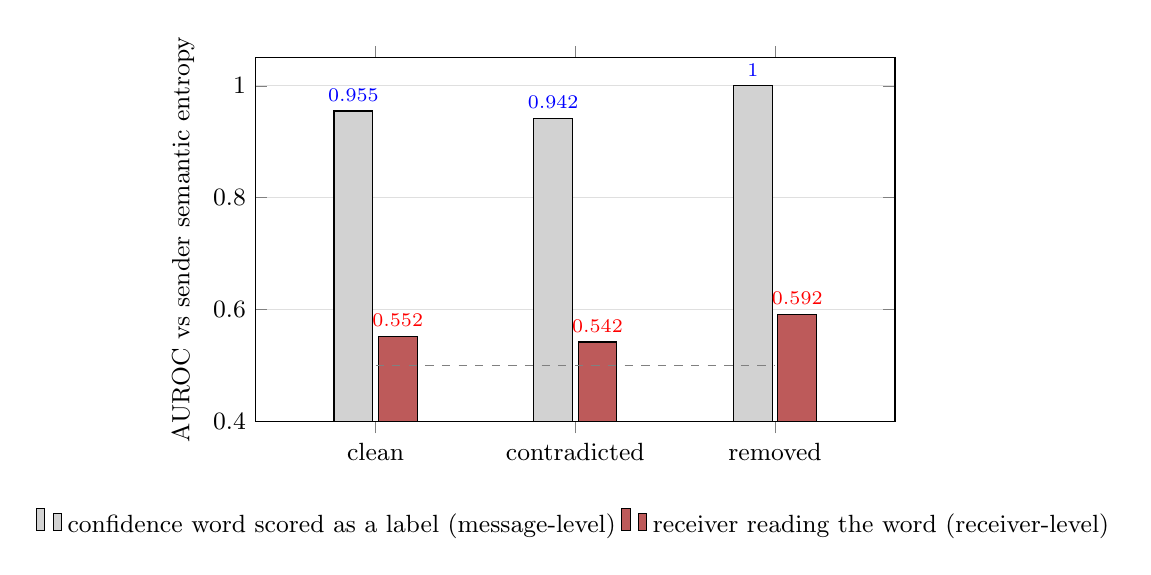
\begin{tikzpicture}
\begin{axis}[
  ybar, bar width=14pt, width=0.8\textwidth, height=6.2cm,
  ymin=0.4, ymax=1.05, % axis limit so the 1.000 bar label fits; not data
  ylabel={AUROC vs sender semantic entropy},
  symbolic x coords={clean, contradicted, removed}, xtick=data,
  enlarge x limits=0.3, ymajorgrids, grid style={gray!25},
  legend style={at={(0.5,-0.22)}, anchor=north, legend columns=2, draw=none, font=\small},
  nodes near coords, nodes near coords style={font=\scriptsize}, every node near coord/.append style={/pgf/number format/.cd, fixed, precision=3},
  tick label style={font=\small}, label style={font=\small},
]
\addplot+[fill=gray!35, draw=black] coordinates {(clean,0.955) (contradicted,0.942) (removed,1.000)};
\addplot+[fill=betc!70, draw=black] coordinates {(clean,0.552) (contradicted,0.542) (removed,0.592)};
\draw[dashed, gray] (axis cs:clean,0.5) -- (axis cs:removed,0.5);
\legend{confidence word scored as a label (message-level), receiver reading the word (receiver-level)}
\end{axis}
\end{tikzpicture}
\caption{The handle. The same confidence word scored two ways on 377 SQuAD items per variant: directly as a label against the sender's semantic entropy, and through the receiver's first-token entropy after it read the word. Dashed line: chance. Numbers from \texttt{docs/paper/main.tex}, Table 5; the 1.000 on removed passages is a degeneracy of the construction (22\% of items tie at the threshold).}
\label{fig:handle}
\end{figure}

\section{Belief, question, finding, mechanism, remedy}

\emph{Belief.} Text handoffs launder uncertainty; a latent carrier is needed.

\emph{Question.} Message or reader?

\emph{Finding.} Reader, on all three variants: the receiver handed the word sits at the level of the receiver handed nothing, while the word itself scores near 1 (SHOWN item 1; \cref{fig:handle}).

\emph{Mechanism.} For the text arm, read-out. For the cache arm, the entry is ``not localised'': linear probes at four points of the chain (\cref{tab:probes}) do not say where the cache arm loses what it loses, and the parsimonious reading is that evidence crosses and the receiver recomputes (SUGGESTED item 4). \SUGG

\emph{Remedy.} One line. Score the message, then score the reader. Report both. The smallest remedy, as when \citet{darcet2024registers} fixed attention artefacts by adding a few spare tokens rather than a new model: no new model here either, no new objective, one extra number in every table that has a verbal-confidence baseline.

%---------------------------------------------------------------------
\chapter{What an economy of state would need}
\label{ch:economy}

\section{Cost, value, fraud}

Once state can be handed off there is something to trade, and a traded good needs three things: a price, a way to be defrauded, and an institution that makes trade safe when the buyer cannot read the good. \src{goal/GOAL.md} puts it as cost, value, fraud $\to$ price, reputation, audit. This chapter says which of those the repository has measured, with the tag each deserves, and keeps the economy itself where it belongs: in the BET column.

\paragraph{Price.} For this pair the price sheet is already written (\cref{tab:pricesheet}), and its declared expectation is that state clears above text only intra-GPU. Time: the projector takes 24\,ms where the receiver's re-read takes 48\,ms, and over a 1\,Gbps link the 72\,MiB message itself takes about 604\,ms. \SHOWN\ Accuracy: 53.0 F1 against 54.7 for text on SQuAD, 39.9 $\pm$ 2.1 against 45.8 on partitioned HotpotQA. \SHOWN\ The byte arithmetic behind the 72\,MiB is in \cref{ch:cost}.

\paragraph{Fraud.} Confidence laundering would be the fraud: a confident-looking state that is wrong. No fraud has been measured. What is measured is that the receiver reads whatever cache it is given: handed the wrong episode's cache by the experimenter, it answers with the wrong episode's value 63.7\% of the time, and handed the output of a projector trained with a deranged sender it answers at 23.4\%, above chance. \SHOWN\ That is the precondition for fraud, and in \cref{ch:content} the same number is the evidence that the channel is read; there was no adversary, no incentive and no detection task. \BET\ That a buyer is exposed to a sender who exploits it is a bet, and \cref{ch:p-fraud} is the chapter that would test it.

\paragraph{Audit.} The audit primitive is the thing this thesis contributes: score the message, then the reader. It is an audit of a text good today. For a state good the message-level instrument is a linear probe, and the probe bounds what one position carries (.557 / .579), not what the map preserves. \SUGG\ An audit a buyer could run on a cache without the seller's cooperation is a bet (\cref{ch:p-fraud}).

\paragraph{Reputation.} Not measured. A sender whose reliability a buyer can track over time requires a sender whose reliability changes, and the three projector checkpoints in the repository are static. \BET\ The futures document's prediction 11 (a within-family projector loses more than 10 points of retention after a post-training update to the receiver, by 2027-12-31) is the cheapest way to make a sender's reliability move, and \cref{ch:p-loop} folds reputation and drift into one experiment for that reason.

\section{The counter-bet: the wire splits at the weights}

The repository holds a second document that argues against the north star. \src{docs/agent-communication-futures-2026-09-21.md} predicts that dense latent channels will run inside a shared-weights boundary and that text, signed and rewritten into a standard form, will cross every organisational boundary, less because of engineering than because of law: recordkeeping, liability, privacy and antitrust rules all assume a message someone can read. Its fifteen dated predictions mature between 2027 and 2030. Three of them bear directly on this program and are listed in the BET box at the front: prediction 11 on drift, prediction 8 on multi-agent gains without private information, prediction 3 on cross-vendor latent state in production.

If the predictions hold, the population studied here is one owner's models: a defensible thesis, and not the agent economy of the north star's third sentence. The disagreement is not resolved here. It is scheduled: \cref{ch:p-loop} runs the drift test that prediction 11 names, and \cref{ch:horizon} records the date on which each prediction is scored.

\section{What this document does not claim}

Nothing here says a KV cache is the right protocol for a population of models; at 72\,MiB per message it is a measurement instrument, not a deployment, and the one experiment that would make it worth its bytes, a task where the sender's state and not its passage is the point, has not been exhibited. Nothing here says the sender's uncertainty crosses the channel as such; the within-item test licenses ``the receiver's confidence moves because of the cache's content'' and no more.

%=====================================================================
\part{What we established}
\label{part:established}
%=====================================================================

\noindent Every number here has a control in the same table.

\chapter{Content transfer and its controls}
\label{ch:content}

\begin{figure}[h]
\centering
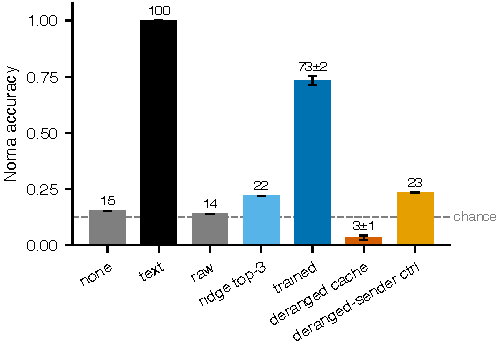
\includegraphics[width=0.72\textwidth]{fig_arms.pdf}
\caption{Only the trained projector reads the cache: it sits far above chance (12.5\%, dashed), the wrong episode's cache below it, the deranged-sender projector near it. Noma 6-name variant, $n = 300$; ``trained'' and ``deranged cache'' are the mean over three training seeds, bars one standard deviation; the deranged-sender control is the \emph{project} arm of the projector trained with a deranged sender ($n = 1000$, 8-name variant).}
\label{fig:arms}
\end{figure}

\section{Why the instrument comes first}

Before the receiver's confidence can track the sender's, the cache must carry the passage. Every later chapter stands on this one, and so does the audit: a message-level signal for the cache is only meaningful if the cache is a channel. The audits of \citet{2608.04893} and \citet{2607.26773} set the bar. The first finds that on natural benchmarks most of a relayed cache's gain is receiver-side computation (MedQA: $+0.4$ of $+14.7$ points is content-specific), and that content transfer appears only when the receiver needs sender-private information. The second decomposes a latent channel's effect into ``sender content'' and ``any message present.'' The binding test, the derange arm and the deranged-sender projector are built for those two objections.

\section{The binding test}

\begin{table}[h]
\caption{Binding transfer, 8 names $\times$ 8 values, $n = 1000$ episodes, chance 12.5\%. All entries are percentages. ``follow'' is the rate at which the receiver, handed the deranged cache, answers with the other episode's value; ``content'' is project $-$ derange.}
\label{tab:main}
\vskip 0.1in
\begin{center}
\begin{small}
\begin{tabular}{lccccccc}
\toprule
projector & none & text & raw & project & derange & follow & content \\
\midrule
ridge top-3 (closed form)          & 10.6 & 100 & 14 & 21.7 & 11.4 & 18.2 & 10.3 \\
$+$ residual, 1500 steps           & 10.6 & 100 & 14 & \textbf{63.0} & 4.6 & \textbf{63.7} & 58.4 \\
residual, deranged sender          & 10.6 & 100 & 14 & 23.4 & 11.3 & 22.7 & 12.1 \\
\bottomrule
\end{tabular}
\end{small}
\end{center}
\vskip -0.1in
\end{table}

Each episode assigns one of eight single-token values to eight nonce names (``Noma is amber. Vela is indigo.\ \ldots''). Only the sender reads the facts. The receiver is asked ``What colour is Vela?'' and the eight values are scored. On the 8-name test (\cref{tab:main}) the trained projector reaches 63.0\% against chance 12.5 and the wrong episode's cache 4.6. \SHOWN\ Handed the wrong episode's cache the receiver answers with the wrong episode's value 63.7\% of the time, and its accuracy falls below chance: it is not ignoring the cache, it is reading it. Matching shape alone (\emph{raw}) does nothing (14\%). The easier 6-name variant ($n = 300$), used for the seeds, the ablations and \cref{fig:arms}, gives 71.3 / 73.0 / 75.3\% over three training seeds (mean 73.2, sd 2.0). \SHOWN\ The same protocol with cities and animals (8 names, $n = 500$) gives 61.8\% and 67.2\%, and padding the facts with up to 512 filler tokens does not reduce accuracy (\cref{ch:pairs}).

Two ablations on the 6-name variant say where the recipe's accuracy comes from (\cref{app:methods}): freezing the ridge and training only the residual gives 59.0\%, so letting the linear map move during training is worth about 14 points; replacing the correlation-selected top-3 source layers with the aligned-layer map gives 32.7\%, so which sender layers feed each receiver layer is the largest design choice. \SHOWN

\section{The deranged-sender projector}

A projector trained with the identical recipe but with the sender reading text unrelated to the receiver's continuation cannot learn a content channel, only a soft prompt. It reaches 23.4\% on the 8-name binding test (\cref{tab:main}, row 3). It is not content-free: its ridge base is weakly content-dependent (ridge alone 21.7\%), so it controls for the \emph{learned} part only. \SHOWN\ This is the ``any message present'' term of \citet{2607.26773}, isolated for a trained map.

\section{Where the binding lives}

\begin{table}[h]
\caption{Where the binding lives. Only the second half of the network carries it, and no six-layer band suffices: this episode's mapped cache is injected into the named band of receiver layers, the deranged episode's elsewhere. 8-name variant, $n = 500$; ``all'' is \cref{tab:main}'s $n = 1000$ row. Accuracy in percent; provenance note in \cref{app:repro}.}
\label{tab:layers}
\vskip 0.1in
\begin{center}
\begin{footnotesize}
\begin{tabular}{lcccccccc}
\toprule
layers   & 0--5 & 0--11 & 0--17 & 12--23 & 24--35 & 30--35 & 18--35 & all \\
\midrule
accuracy & 7.2 & 8.0 & 10.4 & 28.6 & 30.8 & 7.6 & 51.8 & 63.0 \\
\bottomrule
\end{tabular}
\end{footnotesize}
\end{center}
\vskip -0.1in
\end{table}

The first half of the network carries nothing usable on its own, the second half alone carries most of it, and no six-layer band suffices (\cref{tab:layers}, plotted in \cref{fig:distlayers}). \SHOWN\ The binding is read out from a distributed set of later layers. The filler used to complete the cache in these runs is the deranged episode's cache, a plausible but wrong state; \cref{ch:cost} repeats the pruning under a neutral filler and gets the same collapse.

\section{Retention cannot tell a channel from a prompt}

\begin{table}[h]
\caption{Continuation retention is the wrong headline. Retention $= (\mathrm{loss}_{\text{none}} - \mathrm{loss}_{\text{project}}) / (\mathrm{loss}_{\text{none}} - \mathrm{loss}_{\text{oracle}})$ on 128 fresh held-out sequences; the second column swaps the sender's text at test time.}
\label{tab:retention}
\vskip 0.1in
\begin{center}
\begin{small}
\begin{tabular}{lcc}
\toprule
projector & retention & \shortstack{retention, sender\\text deranged} \\
\midrule
ridge top-3                          & $-0.30$ & $-0.66$ \\
$+$ residual                         & 1.23    & 0.31 \\
residual, deranged sender & 0.77    & 0.72 \\
\bottomrule
\end{tabular}
\end{small}
\end{center}
\vskip -0.1in
\end{table}

Following the closed-form-map literature \citep{2608.03893} the paper also reports retention (\cref{tab:retention}; \cref{fig:retention}). Theirs is an accuracy ratio; ours is the fraction of the continuation-loss gap recovered on 128 fresh held-out sequences deduplicated against training text (on 256 such sequences: 1.19 for the trained projector, $-0.38$ for the ridge), so the table critiques our own metric, not theirs. The deranged-sender projector recovers 77\% of the oracle gap, and almost all of it (0.72) survives when its input is deranged at test time. The trained projector's 1.23 decomposes into about 0.3 of the same prompt-like effect and about 0.9 that disappears when the sender's text is swapped. \SHOWN\ Retention above 1 is not evidence of communication, as \citet{2608.04893} objected; the binding test with its derange arm is. The finding is a positive artefact: a metric that cannot tell a channel from a prompt, and a test that can.

\begin{figure}[h]
\centering
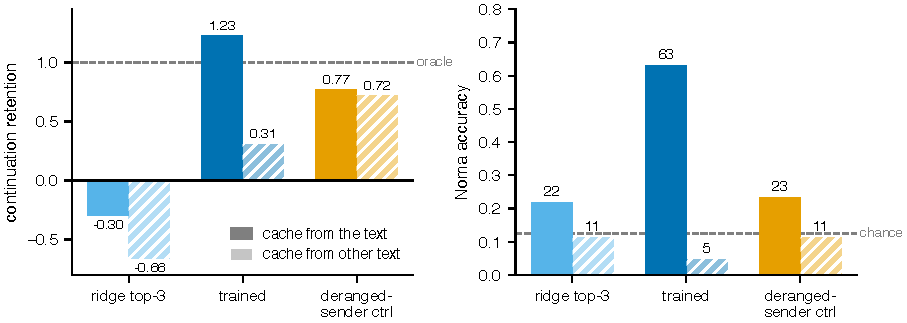
\includegraphics[width=0.8\textwidth]{fig_retention.pdf}
\caption{Retention and the binding test disagree about the deranged-sender control. Left: continuation retention on 128 fresh held-out sequences for the three projectors, with the sender reading the true prefix (solid) or a swapped one (hatched). Right: Noma accuracy for the same three projectors ($n = 1000$, 8-name variant), \emph{project} arm (solid) and \emph{derange} arm (hatched). Retention ranks the deranged-sender projector at 0.77, most of which survives a swapped sender; the binding test puts it at chance.}
\label{fig:retention}
\end{figure}

With that established the instrument is calibrated: the cache carries the passage, and any uncertainty signal measured through it is measured through a channel that could in principle carry one.

%---------------------------------------------------------------------
\chapter{Across families, and where the recipe fails}
\label{ch:pairs}

\begin{figure}[h]
\centering
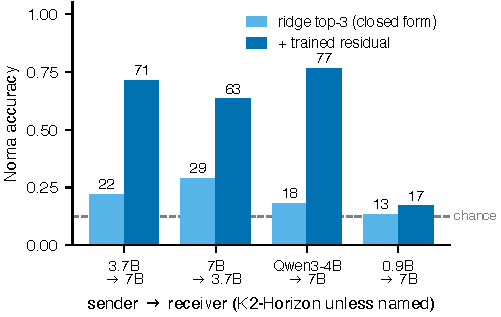
\includegraphics[width=0.52\textwidth]{fig_pairs.pdf}
\caption{The recipe works on three pairs, one of them across a family boundary (Qwen3-4B), and not on the fourth (K2-0.9B, which differs in vocabulary, layer count and head dimension at once). Noma accuracy (\emph{project} arm) for the closed-form ridge map and the trained projector, $n = 300$, 6-name variant; dashed line: chance.}
\label{fig:pairs}
\end{figure}

\section{Other attributes and reversed roles}

\begin{table}[h]
\caption{Binding transfer with city and animal attributes ($n = 500$, 8 names) and with the roles reversed (7B sender, 3.7B receiver; 6 names, $n = 300$).}
\label{tab:attrs}
\vskip 0.1in
\begin{center}
\begin{small}
\begin{tabular}{llcccc}
\toprule
setting & projector & none & project & derange & follow \\
\midrule
city   & ridge top-3            & 14.2 & 19.8 & 11.8 & 18.4 \\
city   & trained                & 14.2 & 61.8 & 6.4  & 60.2 \\
city   & deranged-sender ctrl   & 14.2 & 15.4 & 11.4 & 18.6 \\
animal & ridge top-3            & 12.2 & 12.8 & 12.0 & 11.2 \\
animal & trained                & 12.2 & 67.2 & 5.2  & 64.6 \\
animal & deranged-sender ctrl   & 12.2 & 12.4 & 12.8 & 9.8 \\
reversed & ridge top-3          & 11.7 & 29.0 & 12.3 & 31.3 \\
reversed & trained              & 11.7 & 63.3 & 5.7  & 63.0 \\
\bottomrule
\end{tabular}
\end{small}
\end{center}
\end{table}

The channel is not one attribute and not one-way. With cities and animals in place of colours the trained projector gives 61.8\% and 67.2\% with the deranged-sender control at 15.4\% and 12.4\% (\cref{tab:attrs}). With the roles swapped (7B sender, 3.7B receiver) the ridge map gives 29.0\% and the trained projector 63.3\%, with the deranged cache at 5.7\% and a 63\% follow rate: the same pattern at slightly lower accuracy. \SHOWN\ The reverse map matters later: it is the return path that \cref{ch:p-return} would train on.

\section{Four pairs, one recipe}

\begin{table}[h]
\caption{Four sender--receiver pairs, same recipe. Noma 6-name variant, $n = 300$, chance 12.5\%; percentages. ``proj.'' is the \emph{project} arm, ``der.'' the \emph{derange} arm, ``follow'' the follow rate. SQuAD F1 is for the trained projector ($n = 300$; text ceiling 54.7). K2-Horizon unless named. Qwen3-4B row: proj.\ and F1 are mean $\pm$ sd over three training seeds (76.7 / 70.3 / 68.0; F1 48.0 / 51.9 / 44.9); der.\ is the worst seed, follow is seed 0. The raw arm is undefined for K2-0.9B (head dimension 64).}
\label{tab:pairs}
\vskip 0.1in
\begin{center}
\begin{footnotesize}
\begin{tabular}{lcccccccc}
\toprule
& & \multicolumn{3}{c}{ridge top-3} & \multicolumn{3}{c}{$+$ trained residual} & \\
\cmidrule(lr){3-5}\cmidrule(lr){6-8}
sender $\rightarrow$ receiver & raw & proj. & der. & follow & proj. & der. & follow & F1 \\
\midrule
3.7B $\rightarrow$ 7B    & 14.0 & 22.0 & 10.7 & 30.3 & \textbf{71.3} & 4.3 & 71.7 & 53.0 \\
7B $\rightarrow$ 3.7B    & 11.7 & 29.0 & 12.3 & 31.3 & \textbf{63.3} & 5.7 & 63.0 & --- \\
Qwen3-4B $\rightarrow$ 7B & 15.7 & 18.0 & 13.0 & 17.0 & \textbf{71.7} $\pm$ 4.5 & $\le 4.7$ & 80.3 & 48.3 $\pm$ 3.5 \\
0.9B $\rightarrow$ 7B    & n/a  & 13.3 & 13.0 & 10.7 & 17.0 & 14.0 & 11.3 & 24.2 \\
\bottomrule
\end{tabular}
\end{footnotesize}
\end{center}
\end{table}

With Qwen3-4B as the sender (matched KV geometry, different vocabulary and pre-training; receiver positions aligned to sender tokens by character offsets) the same recipe gives 71.7 $\pm$ 4.5\% over three seeds and 48.3 F1 (\cref{tab:pairs}). \SHOWN\ Cross-family transfer is as strong as within-family on the binding test and within 7 F1 on passages, and the linear map alone does nothing across families (18.0\%).

\section{Where it fails}

For K2-Horizon-0.9B, which differs from the receiver in vocabulary, layer count and head dimension (64) at once, the trained projector reaches 17.0\% against a deranged 14.0\%, and 24.2 F1 (\cref{tab:pairs}). \SHOWN\ This parameterisation fails on that pair. Which of the three differences matters is untested, and cross-head maps exist in other work, so the failure is of this recipe, not of the pair; \cref{ch:failed} returns to it as a finding, and \cref{ch:p-channel} says what a second data point would cost.

\section{Distance}

\begin{table}[h]
\caption{Noma accuracy (\emph{project} arm) versus filler tokens between facts and question. 8-name variant; $n = 1000$ at pad 0, $n = 500$ otherwise.}
\label{tab:distance}
\vskip 0.1in
\begin{center}
\begin{small}
\begin{tabular}{lccccc}
\toprule
projector & 0 & 64 & 128 & 256 & 512 \\
\midrule
ridge top-3          & 21.7 & 22.2 & 22.4 & 22.8 & 24.2 \\
trained              & 63.0 & 61.0 & 57.0 & 62.4 & 68.8 \\
deranged-sender ctrl & 23.4 & 25.0 & 19.8 & 18.2 & 13.8 \\
\bottomrule
\end{tabular}
\end{small}
\end{center}
\end{table}

Padding the facts with neutral filler so that the question is 64 / 128 / 256 / 512 tokens after them gives 61.0 / 57.0 / 62.4 / 68.8\% (\cref{tab:distance}, \cref{fig:distlayers}). No decay; the best value is at the training prefix length of 512. \SHOWN

\begin{figure}[h]
\centering
\begin{subfigure}{0.48\textwidth}
\centering
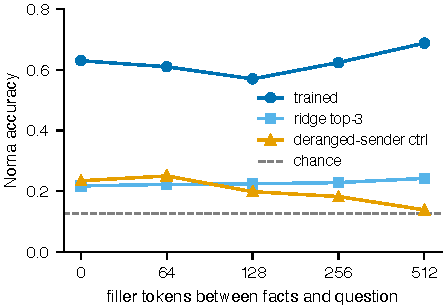
\includegraphics[width=\linewidth]{fig_distance.pdf}
\caption{Accuracy against filler tokens between the facts and the question (8-name variant; $n = 1000$ at 0, $n = 500$ otherwise).}
\end{subfigure}\hfill
\begin{subfigure}{0.48\textwidth}
\centering
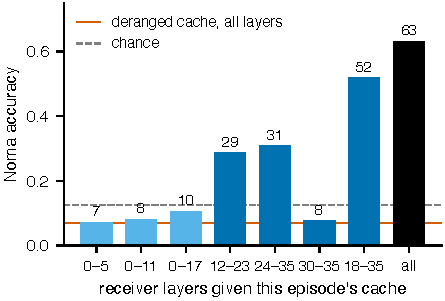
\includegraphics[width=\linewidth]{fig_layers.pdf}
\caption{Accuracy when only the labelled band of receiver layers receives this episode's mapped cache (the deranged episode's cache fills the rest; \cref{tab:layers}). Solid line: the deranged cache in all layers; dashed: chance.}
\end{subfigure}
\caption{Distance sweep and layer-band injection.}
\label{fig:distlayers}
\end{figure}

The one failure in the repository is the one pair with mismatched KV geometry, and the one cross-family success is the pair with matched geometry. Whether geometry is the cause is untested on two data points; it is \cref{ch:p-channel}'s hypothesis, with its kill written there. \SUGG

%---------------------------------------------------------------------
\chapter{Real passages and different contexts}
\label{ch:passages}

\begin{figure}[h]
\centering
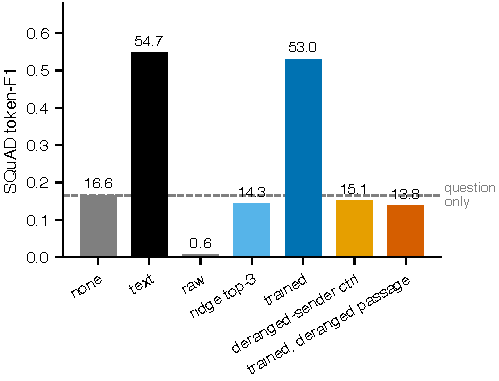
\includegraphics[width=0.72\textwidth]{fig_qa.pdf}
\caption{The mapped cache sits within two F1 of the receiver reading the passage itself, and every control (ridge map, deranged-sender projector, the wrong passage's cache) at or below the question-only floor (dashed). SQuAD token-F1 by arm, $n = 300$.}
\label{fig:qa}
\end{figure}

\section{SQuAD}

\begin{table}[h]
\caption{Real passages: SQuAD v1.1 validation, $n = 300$ (600 for the trained projector). Token-F1 against the gold spans; mean gold log-probability per token.}
\label{tab:qa}
\vskip 0.1in
\begin{center}
\begin{small}
\resizebox{\linewidth}{!}{%
\begin{tabular}{lccccccc}
\toprule
receiver sees & none & text & raw & ridge & trained & \shortstack{deranged-\\sender ctrl} & \shortstack{trained,\\derange arm} \\
\midrule
F1 & 16.6 & 54.7 & 0.6 & 14.3 & \textbf{53.0}\,(51.8) & 15.1 & 13.8 \\
gold log-prob / token & $-3.57$ & $-0.90$ & $-11.2$ & $-3.88$ & $-1.74$ & $-3.77$ & $-4.18$ \\
\bottomrule
\end{tabular}}
\end{small}
\end{center}
\vskip -0.1in
\end{table}

The same projectors, never trained on questions, applied to SQuAD v1.1 validation: the sender reads the passage ($\le 512$ tokens), the receiver reads only the question and answers greedily ($\le 8$ tokens, stopped at newline), token-F1 against the gold spans. On F1 the trained projector recovers 96\% of the gap between question-only and reading the passage (53.0 at $n = 300$; 51.8 at $n = 600$); on gold log-probability it recovers 69\% (\cref{tab:qa}). \SHOWN\ The wrong passage's cache (13.8), the ridge map (14.3) and the deranged-sender projector (15.1) all sit at or below question-only (16.6). On passages, as on the binding test, the channel carries content, not a bias toward answering. The gap between the F1 recovery and the log-probability recovery is the first sign of something \cref{ch:uncertainty} measures directly: the cache path answers nearly as well as the text path and is less confident while doing it.

\section{Different contexts: HotpotQA}

\begin{table}[h]
\caption{HotpotQA bridge questions, $n = 400$. Sender and receiver each hold one of the two supporting paragraphs; the receiver always reads its own paragraph and the question. Token-F1; the mapped cache is mean $\pm$ sd over three training seeds (37.9 / 39.7 / 42.1), the deranged cache their range.}
\label{tab:hotpot}
\vskip 0.1in
\begin{center}
\begin{small}
\begin{tabular}{lc}
\toprule
receiver additionally gets & F1 \\
\midrule
nothing (own paragraph $+$ question)        & 30.1 \\
the sender's paragraph as text              & 45.8 \\
the sender's paragraph as a mapped cache    & \textbf{39.9} $\pm$ 2.1 \\
a deranged mapped cache                     & 29.9--32.1 \\
the sender's paragraph through the ridge map & 26.3 \\
a zero cache                                & 20.9 \\
\bottomrule
\end{tabular}
\end{small}
\end{center}
\end{table}

This is the setting of \citet{2605.22863} and the one setting in the repository where the sender holds evidence the receiver lacks, which \citet{2608.04893} identify as the only condition under which relayed caches carry content on natural tasks. The receiver with its own paragraph and the question reaches F1 30.1; with both paragraphs as text 45.8; with its own paragraph plus the sender's mapped cache 37.9 / 39.7 / 42.1 over the three training seeds (mean 39.9, sd 2.1), 63\% of the gap, while the deranged cache gives 29.9--32.1 (no help), the ridge map 26.3 and a zero cache 20.9 (\cref{tab:hotpot}). \SHOWN\ The channel carries the \emph{other} paragraph, and only the trained map does. The cache costs 5.9 F1 against text here, the number \cref{ch:p-loop}'s price sheet has to beat.

%---------------------------------------------------------------------
\chapter{What the message costs}
\label{ch:cost}

\begin{figure}[h]
\centering
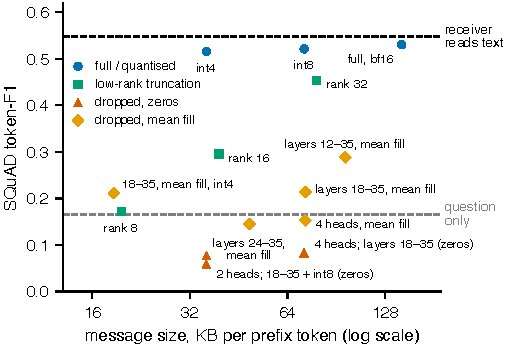
\includegraphics[width=0.55\textwidth]{fig_cost.pdf}
\caption{One free move, quantisation, and no other: every way of cutting the message below a quarter of its size cuts the content with it. Message size against SQuAD F1 for every compression of the mapped cache in the zero- and mean-fill sweep ($n = 300$); the two ``zeros'' points at 72 and 36 KB each hide two coincident specs.}
\label{fig:cost}
\end{figure}

\section{Bytes and time}

\begin{table}[h]
\caption{What the message costs. Bytes per prefix token of the mapped cache (512-token SQuAD passages; ``KB'' $= 1024$ bytes). Noma: 6-name variant, $n = 300$, seed-2 projector. ``filler'' fills the untransmitted layers or heads with the receiver's own cache of a neutral text of the same length. The full sweep, including zero and mean-vector fills and smaller projectors, is in \cref{tab:compress}.}
\label{tab:cost}
\vskip 0.1in
\begin{center}
\begin{footnotesize}
\begin{tabular}{lccc}
\toprule
message & KB / token & Noma & SQuAD F1 \\
\midrule
full mapped cache, bf16 & 144 & 75.3 & 53.0 \\
int4 fake-quantised     & 36  & 75.0 & 51.6 \\
layers 18--35 only, filler elsewhere & 72 & 28.7 & 16.1 \\
4 of 8 heads, filler elsewhere       & 72 & 26.7 & 12.8 \\
\bottomrule
\end{tabular}
\end{footnotesize}
\end{center}
\vskip -0.1in
\end{table}

One move is free, quantisation; every other cut below a quarter of the bytes cuts the content with it. The full mapped cache is 36 layers $\times$ 8 heads $\times$ 2 $\times$ 128 $\times$ bf16 $=$ 144\,KB per token, 72\,MiB for a 512-token prefix, against about 1\,KB of text; the projector has 151\,M parameters. \SHOWN\ Int4 holds both columns of \cref{tab:cost} at a quarter of the bytes, but as fake quantisation, not a packed transport. Dropping layers collapses transfer even when the untransmitted layers hold the receiver's own cache of a neutral text, a valid episode-free state (\cref{tab:cost}, row 3); dropping heads collapses it the same way (row 4); zero and mean-vector fills agree (\cref{tab:compress}), so the loss is missing content, not broken attention, and with this projector the message cannot be cut by layers. \SHOWN\ Low-rank truncation keeps the 6-name binding test and loses passages (\cref{tab:compress}, rank rows).

Latency on one A100: the receiver re-reading 512 tokens takes 48\,ms, the projector 24\,ms. But at 72\,MiB per message a 1\,Gbps link needs about 604\,ms (int4: about 151\,ms) against 24\,ms of receiver compute saved, so the compute advantage does not carry over to a network handoff at this size. \SHOWN\ A reader who can get the sender's uncertainty by re-reading 1\,KB of text should; the channel is worth its bytes only where the sender's state, not its passage, is the point, and the paper has not exhibited such a case. That sentence is the deployment limit, and \cref{ch:p-loop} is built around it.

\section{The full sweep}

\begin{table}[h]
\caption{Every compression of the seed-2 projector's mapped cache. KB per token is for 512-token SQuAD passages; low-rank truncation and mean-vector fill have a per-sequence overhead, so their per-token size depends on sequence length (for the 29-token Noma facts, rank 32 exceeds the full cache). Noma: 6-name variant, $n = 300$, percent; SQuAD: $n = 300$, token-F1. ``filler'' rows fill the untransmitted layers or heads with the receiver's own cache of a neutral text of the same length.}
\label{tab:compress}
\vskip 0.1in
\begin{center}
\begin{footnotesize}
\begin{tabular}{lcccc}
\toprule
spec & KB / token & Noma project & Noma derange & SQuAD F1 \\
\midrule
none (full, bf16)                       & 144  & 75.3 & 2.3  & 53.0 \\
int8                                    & 72   & 76.0 & 2.7  & 52.1 \\
int4                                    & 36   & 75.0 & 3.7  & 51.6 \\
rank 32                                 & 78.7 & 75.0 & 2.3  & 45.3 \\
rank 16                                 & 39.3 & 75.0 & 2.3  & 29.6 \\
rank 8                                  & 19.7 & 51.7 & 7.0  & 17.2 \\
layers 18--35, zeros                    & 72   & 24.3 & 9.7  & 8.3 \\
layers 18--35, zeros, int8              & 36   & 24.7 & 9.7  & 7.8 \\
4 heads, zeros                          & 72   & 25.7 & 8.7  & 8.2 \\
2 heads, zeros                          & 36   & 22.3 & 9.7  & 5.9 \\
layers 12--35, mean fill                & 96.4 & 35.0 & 11.0 & 28.8 \\
layers 18--35, mean fill                & 72.7 & 33.7 & 11.7 & 21.4 \\
layers 18--35, mean fill, int4          & 18.7 & 33.3 & 11.7 & 21.1 \\
layers 24--35, mean fill                & 48.9 & 29.3 & 12.0 & 14.5 \\
4 heads, mean fill                      & 72.7 & 23.0 & 11.3 & 15.3 \\
layers 12--35, filler                   & 96   & 30.7 & 11.7 & 18.9 \\
layers 18--35, filler                   & 72   & 28.7 & 12.0 & 16.1 \\
layers 18--35, filler, int4             & 18   & 30.0 & 11.7 & 16.9 \\
layers 24--35, filler                   & 48   & 25.3 & 10.0 & 13.3 \\
4 heads, filler                         & 72   & 26.7 & 10.0 & 12.8 \\
\midrule
projector bottleneck 32 (70\,M params) & 144 & 64.3 & 5.7 & 53.7 \\
projector bottleneck 16 (62\,M params) & 144 & 61.3 & 7.7 & 51.6 \\
\bottomrule
\end{tabular}
\end{footnotesize}
\end{center}
\end{table}

A projector with bottleneck 32 has 70\,M parameters and keeps SQuAD F1 (53.7) while losing 9 points on the binding test (64.3\%); bottleneck 16 (62\,M) gives 61.3\% and 51.6 F1. The filler rows are the structural null: the receiver's own cache of a neutral text is a valid, episode-free state, so a collapse under it is missing content rather than broken attention. \SHOWN\ Three nulls (zeros, mean fill, filler) agree, which is why \cref{ch:failed} files layer pruning under findings rather than under things still worth trying with this projector.

%---------------------------------------------------------------------
\chapter{Uncertainty: how much survives each handoff}
\label{ch:uncertainty}

\begin{figure}[h]
\centering
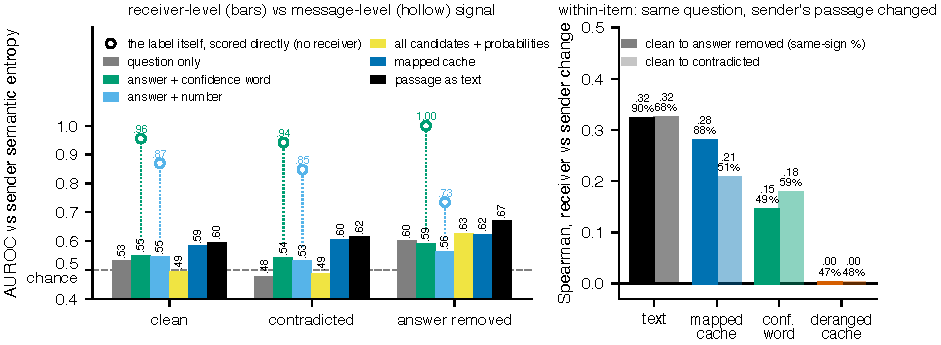
\includegraphics[width=0.95\textwidth]{fig_audit.pdf}
\caption{The read-out gap as a vertical distance: the hollow markers for the word and the number (the label scored directly) sit far above their bars (the receiver that read it), and the cache, which has no label and no marker, sits level with the text. Left: AUROC of the receiver's first-token entropy against the sender's semantic entropy, 377 items, six handoffs per passage variant. Right: within-item intervention, the question held fixed and the sender's passage changed; bars are the Spearman correlation between the receiver's entropy change and the sender's semantic-entropy change, annotated with the same-sign rate, which is bounded by the 91.5\% of items on which the sender's entropy rises.}
\label{fig:audit}
\end{figure}

\section{The protocol}

Following the knowledge-conflict and semantic-entropy protocols \citep{longpre2021entity,xie2023adaptive,farquhar2024detecting}, each SQuAD item gets three passages: \emph{clean}, \emph{contradicted} (one fluent sentence asserting a counter-answer, written by the 375B judge and kept only if DeBERTa-MNLI says it entails the counter-answer and not the gold: 587 of 941 survive), and \emph{removed} (the gold sentence deleted). The 377 items (344 distinct passages) on which the receiver reading the clean passage reaches token-F1 $\ge .5$ are kept. The sender's uncertainty is its semantic entropy (SE) over 10 sampled answers (mean 0.98 / 1.18 / 1.96 over the 377 kept items on the three variants, so the sender does notice); the target is SE thresholded at its median per variant. Ten samples make SE coarse: 38 / 40 / 28 distinct values per variant, and on removed passages 22\% of items sit exactly at the threshold. The receiver's uncertainty is its entropy at the first answer token.

Four messages. Two are functions of the passage alone, $M = f(c)$, with the question unseen by the sender: \emph{text} and \emph{mapped cache}. Two require the sender to answer the question, $M = f(c, q)$: \emph{verbal} (the sender's greedy answer and ``confidence: high / medium / low'') and its variants with a number (the sender's sample agreement, e.g.\ ``0.8'') or the full candidate list (every answer cluster with its sampled frequency). The confidence word is an oracle label built from the sender's \emph{actual} SE terciles, favourable to the text channel; the sender does not verbalise its own confidence. The receiver's prompt is a plain completion with no chat template, no few-shot examples and no instruction to hedge; it was not ablated, and \cref{ch:failed} says what that leaves open. Content-free controls per variant: a deranged cache (another item's), a zero cache, a moment-matched random cache, and question only. \Cref{app:protocol} has the definitions in full.

\section{The table}

\begin{table}[h]
\caption{Sender uncertainty through each handoff; 377 SQuAD items on which the receiver reading the clean passage reaches token-F1 $\ge .5$. AUROC is of the receiver's first-token entropy against the sender's semantic entropy (thresholded at its median per variant); the drop ratio is the receiver's $P(\text{gold})$ loss from clean to removed relative to the text path's. The two ``scored directly'' rows are the message-level signal: the label itself ranked against the same target, with no receiver. Two projectors trained with uncertainty objectives are in \cref{tab:negative}.}
\label{tab:confidence}
\vskip 0.1in
\begin{center}
\begin{small}
\resizebox{\textwidth}{!}{%
\begin{tabular}{lcccc}
\toprule
receiver sees & \shortstack{$P(\text{gold})$\\clean / contra. / removed} & \shortstack{entropy\\clean / removed} & \shortstack{AUROC vs sender SE\\clean / contra. / removed} & drop ratio \\
\midrule
text                                & .437 / .290 / .162 & 1.14 / 3.03 & .597 / .615 / .671 & 1 (def.) \\
text $+$ answer $+$ confidence word (verbal) & .253 / .193 / .171 & 2.88 / 2.80 & .552 / .542 / .592 & .30 \\
text $+$ answer $+$ numeric confidence (sample agreement, e.g.\ ``0.8'') & .258 / .197 / .170 & 2.93 / 2.93 & .548 / .532 / .563 & .32 \\
text $+$ all candidate answers with their sampled probabilities & .264 / .210 / .144 & 2.68 / 2.63 & .495 / .489 / .626 & .44 \\
\textbf{mapped cache}               & .279 / .249 / .130 & 1.78 / 3.16 & \textbf{.585 / .605 / .624} & \textbf{.54} \\
deranged cache                      & .105 / .106 / .105 & 3.88 / 3.88 & .536 / .488 / .564 & 0 \\
zero cache                          & .034 / .033 / .037 & 6.41 / 6.18 & .496 / .481 / .502 & 0 \\
moment-matched random cache         & .005 / .004 / .005 & 7.24 / 7.30 & .457 / .472 / .580 & 0 \\
question only                       & .127               & 3.69        & .532 / .479 / .603 & 0 \\
\midrule
\multicolumn{5}{l}{\emph{message-level signal (no receiver)}} \\
confidence word, scored directly as a label & --- & --- & .955 / .942 / 1.000 & --- \\
numeric confidence, scored directly & --- & --- & .870 / .848 / .735 & --- \\
\bottomrule
\end{tabular}}
\end{small}
\end{center}
\vskip -0.1in
\end{table}

\section{Every arm as two rows}

A reader should leave with the split, not the aggregate. \Cref{tab:tworows} rewrites \cref{tab:confidence} that way: a label row, a reader row, and the read-out gap, per arm, with the row in which the loss sits named in prose.

\begin{table}[h]
\caption{Each handoff as a two-level report, clean / contradicted / removed. The read-out gap rows are differences, not measurements: the word's is computed from the unrounded values in \texttt{analysis/cloud/verbal/audit.json} (.9555 $-$ .5518, .9415 $-$ .5422, 1.000 $-$ .5921), the number's from \texttt{night\_a/confidence\_numeric.json} with the same file's label AUROC. The message-level row for the cache is the one-position linear probe of \cref{ch:where}, run on the 587-item set rather than the 377 (clean / removed only), so its gap is not comparable across arms and is written in grey. The candidate-list arm has no label row: its entropy against the sender target is near 1 by construction, as the word's is, and is not computed. Other numbers from \cref{tab:confidence} and \cref{ch:where}.}
\label{tab:tworows}
\vskip 0.1in
\centering
\small
\begin{tabular}{llccc}
\toprule
arm & level & clean & contradicted & removed \\
\midrule
confidence word & message (label) & .955 & .942 & 1.000 \\
                & receiver        & .552 & .542 & .592 \\
                & read-out gap    & .404 & .399 & .408 \\
\midrule
numeric confidence & message (label) & .870 & .848 & .735 \\
                   & receiver        & .548 & .532 & .563 \\
                   & read-out gap    & .322 & .316 & .172 \\
\midrule
mapped cache & message (one-position probe, 587 items) & \textcolor{gray}{.557} & --- & \textcolor{gray}{.579} \\
             & receiver (377 items)                     & .585 & .605 & .624 \\
             & read-out gap                             & \multicolumn{3}{c}{\textcolor{gray}{not localised; see \cref{ch:where}}} \\
\midrule
text (passage) & message & \multicolumn{3}{c}{no label to score} \\
               & receiver & .597 & .615 & .671 \\
\bottomrule
\end{tabular}
\end{table}

For the word and the number the loss sits in the reader row: the label is near-perfect by construction and the receiver reading it is within .07 of question-only on every variant ($+.020$ / $+.063$ / $-.011$). \SHOWN\ For the cache the loss cannot be assigned to a row: the receiver recovers more (.643, by the probe protocol of \cref{ch:where}) than a one-position probe of its message carries (.557), so the message carries more than one position reads, and the entry is ``not localised.'' \SUGG\ For text there is no message-level row at all, which is the point: the passage is not a summary of the sender's belief but the evidence it was formed from, and the receiver forms its own.

\section{Result}

The cache beats every summary of the sender's belief and loses to the passage itself, but only one of those gaps is established. On clean and contradicted passages the ordering of receiver-level signal is text, then the mapped cache, then every summary of the sender's belief; on removed passages the candidate list matches the cache (.626 vs .624) and question-only (.603) beats the word (.592). The cache beats the confidence word by $+.03$ to $+.06$ AUROC, and its drop ratio is .54, that is $(.279 - .130) / (.437 - .162)$, where the word's is .30. Writing the confidence as a number does not help the text channel (.548 / .532 / .563; drop ratio .32), and neither does the strongest text message that can be built from the sender's samples, every answer cluster with its frequency (.495 / .489 / .626; drop ratio .44). \SHOWN

Intervals were computed for three differences, each a paired bootstrap over passages (344 passages, 2,000 resamples). Cache $-$ word excludes zero on contradicted passages ($[.008, .117]$) and not on clean ($[-.027, .094]$) or removed ($[-.024, .086]$); cache $-$ question-only excludes zero on contradicted ($[.065, .180]$) and is borderline on clean ($[-.005, .111]$); cache $-$ text includes zero on clean ($[-.066, .047]$) and contradicted ($[-.064, .047]$) and excludes it on removed ($[-.091, -.002]$), where the text path is above the cache. The direction is consistent; the size is modest and established on one variant of three. \SUGG

\paragraph{The pre-registered criterion was missed.} \src{docs/design-confidence-2026-09-22.md} fixed, before the run, two conditions for proceeding to a claim: (a) cache-arm AUROC against the sender label at or above .70 and above every control by more than its interval; (b) the cache path's confidence drop on removed items at least 50\% of the text path's. The measured cache arm is .585 / .605 / .624, so (a) fails on all three variants; (b) passes, at .54. The same document wrote the fallback reading for that outcome: ``content transfers, uncertainty does not.'' That fallback is what this chapter reports under the words ``evidence crosses and the receiver recomputes,'' and it is why cache $>$ word carries the SUGGESTED tag and not SHOWN, and why the north-star phrase ``uncertainty that travels with it'' is not claimed anywhere in this document. \src{goal/GOAL.md}'s 12-month status line, ``milestone 3 half done (uncertainty survives attenuated),'' is the pre-criterion wording and is reconciled to this paragraph in that file.

\section{Controls, per variant}

The controls do not sit at one level: when the answer is removed the question alone already carries most of the signal (.603), so the cache's real increment is the contradicted variant's $+.126$. An earlier draft that put all controls at one level was corrected by review (\cref{app:reviews}). On clean and contradicted passages they lie at .46--.54 (question only .532 / .479; deranged .536 / .488; random .457 / .472; zero .496 / .481) against the cache's .585 / .605. On removed passages question-only alone gives .603, the random cache .580 and the deranged cache .564 against the cache's .624: the question already carries most of the signal when the answer is gone, and question-only there beats the word (.592). The cache's increment over question-only is therefore $+.053$ on clean, $+.126$ on contradicted and $+.021$ on removed passages, and only the middle one is established. \SHOWN

\section{Behaviour under contradiction and removal}

\begin{figure}[h]
\centering
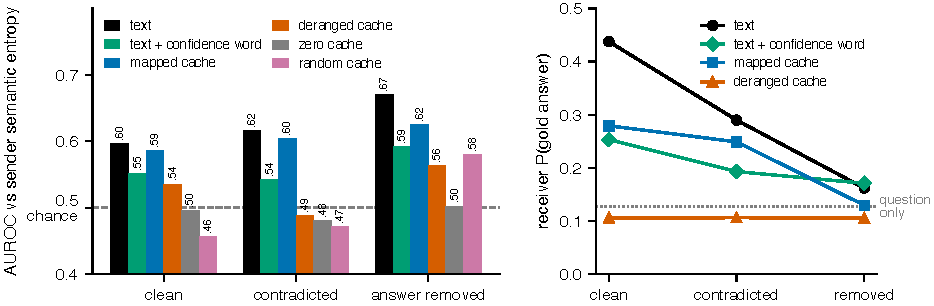
\includegraphics[width=0.8\textwidth]{fig_confidence.pdf}
\caption{Left: AUROC of the receiver's first-token entropy against the sender's semantic entropy, per handoff and passage variant (377 items), including the zero and moment-matched random caches. Right: the receiver's $P(\text{gold})$ from clean to contradicted to removed passages. The cache path is less confident than the text path on clean passages and keeps the original answer ahead under a contradiction.}
\label{fig:confidence}
\end{figure}

The cache path is a damped copy of the text path, not a different reader. When the answer is removed it loses 54\% of the confidence the text path loses and its entropy rises by 73\% of the text path's rise; under a contradiction the text path tips toward the inserted sentence ($P(\text{counter})$ .32 $>$ $P(\text{gold})$ .29) where the cache path keeps the original ahead (.25 $>$ .22); and on clean passages it is less confident throughout ($P(\text{gold})$ .28 vs .44; \cref{fig:confidence}). \SUGG\ Two readings fit this. One is that the map attenuates the evidence, so the receiver sees a blurred passage and moves less; the other is that the map carries the passage and the receiver's own prior weighs more against a cache than against text it can read token by token. The drop ratio cannot separate them, no interval was computed for it, and this is the first place the latent-carrier thesis of \citet{2606.20662} meets a measurement that neither confirms nor refutes it: a receiver whose confidence moves less through state than through text is not what a latent carrier of uncertainty predicts. Which reading holds is the question \cref{ch:where} takes up and leaves open, and \cref{ch:p-uncert}'s pooled probe is built to split it.

%---------------------------------------------------------------------
\chapter{Where the loss occurs}
\label{ch:where}

The word arm's loss is at the reader; the cache arm's is not localised. Three tests say so; two carry a control or an interval; all three were run on 2026-09-25 after the fifth and sixth reviews asked for them (\cref{app:reviews}), so they are checks, not pre-registered predictions, and the expectation written before each result below was written after the numbers existed.

\section{Three tests that the reader discards the label}

\emph{Test 1, expectation.} If the loss on the word arm is in the message, the word scored directly against the sender target will be low, near the receiver's .552. If the loss is in the reader, the word will score high and the receiver low.

\emph{Test 1, result: the label-only audit.} The confidence word is built from the sender's own SE terciles, so scored as a label it predicts the binary target almost perfectly without any receiver: AUROC .955 / .942 / 1.000 on the three variants, the numeric label .870 / .848 / .735 (\cref{tab:confidence}, bottom). \SHOWN\ These numbers are a property of the construction, a tercile split over all 587 items against a median split over the 377 kept items, and the 1.000 on removed passages is a degeneracy: 22\% of items tie at the threshold and the tercile boundary coincides with it. The audit is a sanity check, not a finding; the finding is the other bar: the receiver's first-token entropy after reading that word reaches .552 / .542 / .592. The text channel is not capacity-limited here.

\emph{Test 2, expectation.} If the receiver's confidence moves because of what the sender saw, and not because hard questions make both models uncertain, then changing only the sender's passage (question fixed) will move the receiver's entropy with the sender's through a channel that carries the passage, and will not move it through a cache that shares the question but not the passage.

\emph{Test 2, result: the within-item intervention.} The variants allow a paired test with the question held fixed and only the sender's passage changed (clean $\to$ removed; the sender's SE rises by 0.98 on average). Per item, the Spearman correlation between the receiver's entropy change and the sender's SE change is .280 through the mapped cache, .322 when the receiver reads the text, .146 through the confidence word, and .004 through a cache from another item, which shares the question and rules out the common cause (\cref{fig:audit}, right). \SHOWN\ The same-sign rates (88 / 90 / 49 / 47\%) are weaker evidence than they look: the sender's SE rises on 91.5\% of items, so any arm whose entropy simply rises on removal scores near that ceiling and an arm with no mean shift sits at a coin flip; same-sign measures the mean shift, the Spearman the per-item covariation. Under a contradiction the effect is smaller (cache .208, text .325, word .179, deranged .004). The receiver's confidence moves with what the sender saw, and it moves because of the cache's content. It licenses no more than that: the text path tracks at least as well, so the parsimonious reading is that the evidence crosses and the receiver recomputes its own uncertainty from it.

\emph{Test 3, expectation.} If the reader discards the label, then on passages where the answer is gone, a receiver with no message at all should do no worse than a receiver handed the word.

\emph{Test 3, result: question-only against the word on removed passages.} Question-only reaches .603, the word .592 (\cref{tab:confidence}). \SUGG\ No interval was computed for this pair; it is a direction, .011 wide, and it is counted as such. The label, which scores 1.000 directly on this variant, adds nothing the question did not already give the receiver.

Three tests in agreement, two of them with a control or an interval behind them. The read-out failure is a property of the label channel for this reader, not of handoffs in general. It is also why the capacity argument of the paper's earlier draft (\cref{ch:failed}) cannot be the mechanism of the verbal arm's shortfall: a channel that delivers a .955 label is not the bottleneck.

\section{Shape of the belief}

\msugg Sender SE and receiver first-token entropy are different measurements; a diagnostic closer to the belief itself is the \emph{shape}: per item with at least two sampled answer clusters, the Spearman correlation between the sender's cluster frequencies and the receiver's first-token mass on those candidates. On clean passages ($n = 323$) it is .199 through the mapped cache, .193 from the text, .166 from the explicit candidate list, and .052 / .042 for the deranged cache and question only: there the receiver recovers the sender's alternatives about as well from the cache as from the passage, and no better from a list of them. Under a contradiction ($n = 351$) the order reverses (cache .153, list .201, text .234), and on removed passages every arm is near zero. \SUGG\ No interval was computed for these correlations, and they are small enough that the diagnostic separates arms from the controls, not from each other.

\section{Four-point probes: the cache arm's loss is not localised}

\msugg The probes in \cref{tab:probes} were built to localise the cache arm's loss, and they did not. The instrument was chosen for comparability: the same standardised logistic probe (\citealp{kossen2024sep}; $C = 0.05$, five passage-grouped folds, no inner selection) at four points of the chain, sender state, mapped message, receiver state via cache, receiver state via text, so that a drop between two adjacent points would name the stage at which the sender's uncertainty is lost. They run on the 587 items before the F1 filter, so their AUROCs are not comparable with \cref{tab:confidence}; the numbers are in the table and are not repeated here. A one-position probe of the message was used because the mapped cache has no label and its last prefix position is the one place a fixed-size read-out exists without training a reader; that choice is the weakness named below.

\begin{table}[h]
\caption{Four-point probes against the binary sender-SE target, 587 items, clean / removed. AUROC of a standardised logistic probe with passage-grouped folds. From \texttt{docs/paper/main.tex}, Section 5(d); \texttt{analysis/cloud/night\_a/diag\_unc\_clean.json} and \texttt{diag\_unc\_removed.json}.}
\label{tab:probes}
\vskip 0.1in
\centering
\small
\begin{tabular}{lcc}
\toprule
probed state & clean & removed \\
\midrule
sender, last prompt token, layers 12 / 18 / 24 & .739 & .706 \\
mapped message, last prefix position & .557 & .579 \\
mapped message $+$ question-only receiver state & .563 & .603 \\
receiver after reading the mapped cache & .643 & .563 \\
receiver after reading the text & .650 & .654 \\
receiver, question only & .530 & .591 \\
\bottomrule
\end{tabular}
\end{table}

What the table shows is a chain that is not monotone. The sender's own state is the top of it on both variants; the receiver recovers more through the cache (.643 on clean) than the probed message carries (.557), which cannot happen if the one-position probe measured what the map preserves; and the cache leaves the receiver level with the text on clean passages and below it on removed. \SUGG\ That leaves two readings open. \emph{Map loss}: the projector attenuates the sender's spread, the receiver recomputes from blurred evidence, and the sender-to-receiver drop (.739 to .643) is real. \emph{Probe weakness}: the spread is in the message, distributed over 512 positions, and a probe that reads one of them cannot see it, so the message row is a floor and the drop is an artefact of the instrument. A third confound sits across both: the sender probe saw the question and the mapped message is passage-only, so sender-minus-message mixes question conditioning with map loss. \cref{ch:p-uncert}'s pooled probe over all 512 positions discriminates the first two: if it exceeds .643 on clean passages, probe weakness is the reading and the message carries more than the receiver uses; if it stays at the one-position level, map loss is the reading and the sender side is where the fix belongs. The kill is one-sided and fixed there. For the latent-carrier thesis of \citet{2606.20662} the result as it stands is neutral: a one-position read of the latent carries less about the sender's uncertainty than the sender's own state, and nothing here says whether the rest of the latent carries the difference.

\section{What the analysis licenses}

For the text arm: read-out. For the cache arm: evidence crosses and the receiver recomputes, with the sender's spread crossing as such neither shown nor excluded. The thesis's title claim is therefore about the label, and the cache is in the title only as the contrast that shows the receiver can be moved by a message when the message is the evidence rather than a summary of it. Nothing here says a text handoff cannot carry uncertainty; it says this base receiver, under one completion prompt, does not read the label it was handed.

%=====================================================================
\part{What failed and what it taught}
\label{part:failed}
%=====================================================================

\noindent Each negative here closed a door a later chapter would otherwise have had to open.

\chapter{Six negatives, filed as findings}
\label{ch:failed}

None of the six is an apology; each is tagged with what it established.

\section{The 0.9B pair: a recipe has a domain}

What it taught: the one failure in the repository is the one pair with mismatched KV geometry, and the one cross-family success is the pair with matched geometry (\cref{tab:pairs}). \SHOWN\ The inference from that to ``geometry, not family membership, is what this parameterisation needs'' rests on two data points, and K2-Horizon-0.9B differs from the receiver in three things at once, so which of them matters is untested. \SUGG\ That is why the program treats ``content transfer is a property of the triple'' as a hypothesis with a kill (\cref{ch:p-channel}) rather than a conclusion, and why the retention critique and the cost sweep, not this pair, are what the channel chapter stands on.

\section{Pruning under three null states: the message cannot be cut by layers}

The layer-band table (\cref{tab:layers}) showed the second half of the network alone carries most of the binding; the natural next move was to send only those layers. Under three fills for the untransmitted layers (zeros, the per-layer mean vector, and the receiver's own cache of a neutral text) layers 18--35 give 24.3 / 33.7 / 28.7\% on the 6-name variant and 8.3 / 21.4 / 16.1 F1 (\cref{tab:compress}). \SHOWN\ The fourth review had pointed out that a zero fill dilutes the softmax, so a collapse under zeros could be broken attention rather than missing content; the filler fill is a valid episode-free state, and the collapse survives it. What it taught: with this projector every receiver layer wants its own cache, and the 72\,MiB figure cannot be halved by dropping layers. The by-layer route to a cheaper message is closed for this recipe; training-time layer dropout is the untested alternative.

\section{Low rank: the binding test is too easy to price a message by}

Low-rank truncation of each (positions $\times$ head-dim) matrix at rank 32 and 16 keeps the 6-name binding test at 75.0\% and loses passages (F1 45.3 and 29.6; rank 8: 51.7\% and 17.2 F1). \SHOWN\ What it taught: a compression that passes the binding test can still destroy the passage, so the binding test alone cannot be used to price a message. Every compression row in \cref{tab:compress} carries both columns for that reason, and \cref{ch:p-channel}'s sender catalogue requires both.

\section{Two training objectives that did not move the loss}

\begin{table}[h]
\caption{Two projectors trained with an uncertainty objective (weight 1, 1,000 steps), scored exactly as in \cref{tab:confidence}.}
\label{tab:negative}
\vskip 0.1in
\begin{center}
\begin{small}
\resizebox{\textwidth}{!}{%
\begin{tabular}{lcccc}
\toprule
receiver sees & \shortstack{$P(\text{gold})$\\clean / contra. / removed} & \shortstack{entropy\\clean / removed} & \shortstack{AUROC vs sender SE\\clean / contra. / removed} & drop ratio \\
\midrule
mapped cache (reference, \cref{tab:confidence}) & .279 / .249 / .130 & 1.78 / 3.16 & .585 / .605 / .624 & .54 \\
mapped cache, KL-trained projector  & .272 / .241 / .118 & 2.38 / 3.76 & .590 / .589 / .611 & .56 \\
mapped cache, sender-entropy-matched projector & .247 / .222 / .107 & 2.23 / 3.64 & .596 / .587 / .627 & .51 \\
\bottomrule
\end{tabular}}
\end{small}
\end{center}
\end{table}

If the cache arm's shortfall were an artefact of the projector's training target, changing the target should move it. Two receiver-side objectives did not (\cref{tab:negative}). Adding $\mathrm{KL}(\text{text-path} \,\|\, \text{cache-path})$ on the receiver's next-token distributions (weight 1, 1,000 steps) raises the cache path's entropy everywhere (clean 2.38 vs 1.78) without making it track the sender better (AUROC .590 / .589 / .611; drop ratio .56 vs .54) and costs 2 F1. Matching the receiver's per-token entropy through the cache to the sender's own per-token entropy on the training text holds binding accuracy (72.3\%), drops SQuAD F1 to 45.3, and leaves the uncertainty measures where they were (.596 / .587 / .627; drop ratio .51). \SHOWN\ What it taught: neither target contains the sender's spread. The receiver's own text path does not contain it either, and entropy matching is not belief matching. The untested fix is on the other side of the map: a separate reader $r(m, q)$ trained on the sender's candidate distribution and kept apart from the receiver's own decision. That is \cref{ch:p-uncert}'s pooled reader.

\section{The handoff policy on SQuAD: the trigger works, the task does not pay}

\begin{table}[h]
\caption{Handoff policy on 600 SQuAD items. Top: AUROC of each trigger at predicting the sender's own failures (F1 $< 0.5$). Bottom: F1 of each arm when every item is handed off (rate 1). \texttt{analysis/cloud/cascade/curves.json}.}
\label{tab:policy}
\vskip 0.1in
\begin{center}
\begin{small}
\begin{tabular}{lc}
\toprule
\multicolumn{2}{l}{sender (3.7B) alone: F1 52.2, wrong on 35.5\% of items} \\
\midrule
trigger & AUROC \\
\midrule
probe on the sender's hidden state & \textbf{.749} \\
semantic entropy (10 samples)                 & .689 \\
sample disagreement                           & .683 \\
max-probability                               & .582 \\
entropy                                       & .584 \\
\midrule
receiver (7B) sees & F1 at rate 1 \\
\midrule
the passage as text          & 55.7 \\
the mapped cache             & 51.8 \\
the sender's answer $+$ confidence word & 47.0 \\
\bottomrule
\end{tabular}
\end{small}
\end{center}
\end{table}

\begin{figure}[h]
\centering
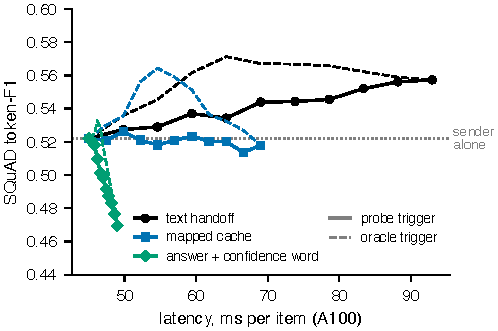
\includegraphics[width=0.55\textwidth]{fig_policy.pdf}
\caption{F1 against latency per item as the handoff rate goes from 0 (sender alone, 45\,ms) to 1, for the three handoff arms under the probe trigger (solid) and an oracle trigger that hands off exactly the sender's failures (dashed). 600 SQuAD items. Only the oracle gains; the probe-triggered text handoff climbs to the receiver's own 55.7, the cache handoff stays flat.}
\label{fig:policy}
\end{figure}

On 600 SQuAD items the 3.7B alone reaches F1 52.2 and gets 35.5\% of items wrong. A logistic probe on its pre-action hidden state (last prompt token, layers 12 / 18 / 24; five-fold, not grouped by passage, $C = 0.1$) predicts those failures with AUROC .749, better than its own semantic entropy (.689), sample disagreement (.683), max-probability (.582) or entropy (.584) (\cref{tab:policy}). \SHOWN\ The same kind of probe on 127 agent steps from 26 runs, nested leave-one-run-out, reaches .876 $[.813, .944]$ at layer 18 against trajectory metadata at .704, and in the shortcut audit the probe alone gives .881, metadata .703, both together .835 (\src{analysis/cloud/nested_3.7b.json}, \src{shortcut_k2-3.7b.json}). \SHOWN\ The sender's state knows when the sender will fail.

But the 7B reading the passage reaches only 55.7, the mapped cache 51.8 and the verbal handoff 47.0 (\cref{fig:policy}): the probe-triggered text handoff climbs from 52.2 to 55.7 as the handoff rate goes to 1, with per-item latency going from 45 to 93\,ms, the cache handoff stays flat near 52, and only an oracle trigger gains (56.4 at rate .4). \SHOWN\ That is the measurement: 3.5 F1 for 48\,ms per item, and nothing from the cache arm. Whether it ``pays'' needs an exchange rate between F1 and milliseconds that this document fixes only in \cref{tab:pricesheet}; the author's reading is that it does not, and the condition that was met is the kill written in \src{docs/design-cascade-2026-09-24.md}, state never beating text at equal cost on any rate. What it taught: the receiver is not enough better than the sender on this task for a handoff of any kind to be worth it, which is a fact about SQuAD and not about the trigger. The policy result waits for a task with a real gap, and \cref{ch:p-loop} refuses to run until that gap has been measured.

\section{The retracted $\log 3$ deduction}

Version 4 of the paper carried a theory box that deduced the text arm's low receiver-level AUROC from a capacity bound: a message that is the argmax of the sender's belief plus a $k$-level label takes at most $|Y|\,k$ values and so carries at most $\log |Y| + \log k$ nats about the belief. The bound is correct and limits information about the \emph{distribution}; it does not limit a detector's AUROC against a thresholded target, and a three-level label reaches .955 against the median split. The step from the bound to the AUROC was invalid, it was never the argument of \citet{2606.20662}, and it was withdrawn on 2026-09-25 after two external reviews said the same thing (\cref{app:reviews}). What it taught: the measurement does the work, and theory enters this document only as a toy that makes a prediction (\cref{sec:readout}), never as a proof that the measurement had to come out that way. What survives of the box is one modest statement: if the receiver's recovered belief is within total variation $\varepsilon$ of the sender's and one-step rewards lie in $[0, R_{\max}]$, acting on the recovered belief loses at most $2 R_{\max} \varepsilon$ in expected reward. That is what a decision test should measure, and no experiment here measures regret.

\section{What would change the claim}
\label{sec:change}

Each limitation below is paired with the cheapest experiment that would close it, and the last one is the experiment that would overturn the main claim.

\begin{itemize}
\item \emph{One projector seed through the confidence protocol.} The three seeds trained for the binding test have not been run through it. Cheapest fix: run them; \src{docs/design-confidence-2026-09-22.md} prices the protocol at one A100 session, under \$15. If the seed sd of cache $-$ word exceeds the .03--.06 effect, the cache-versus-word ordering drops from SUGGESTED to unshown.
\item \emph{One dataset, one sender--receiver pair, one uncertainty measure.} Cheapest fix: the 377-item protocol on the HotpotQA partitioned items, eval-only on cached states.
\item \emph{The four-point probes read one position.} Cheapest fix: a pooled read-out over all 512 prefix positions, with a one-sided kill fixed in advance (\cref{ch:p-uncert}).
\item \emph{The deployment limit.} 144\,KB per token; about 604\,ms per message on a 1\,Gbps link against 24\,ms saved. No experiment closes this; the price sheet of \cref{ch:p-loop} declares where state can clear and where it cannot.
\item \emph{The overturning experiment.} ``The receiver does not read the label'' is a property of one base model under one completion prompt: no prompt ablation, no few-shot examples, no chat template, no instruction-tuned receiver, and the candidate-list arm scoring below question-only on clean passages (.495 vs .532) says the text baselines are not the strongest a competent engineer could build. A receiver whose entropy follows ``confidence: low'', an instruction-tuned or few-shot reader, would erase the contrast. That is the first experiment the program runs (\cref{ch:p-uncert}), because it is the only one that can change the abstract.
\end{itemize}

%=====================================================================
\part{The program}
\label{part:program}
%=====================================================================

\noindent Everything from here is a bet, and every bet has its kill written before its run.

\chapter{The thesis sentence, the price sheet, and the order of the kills}
\label{ch:program}

\section{The sentence, written as a conditional}

\mbet \emph{A small frozen model that predicts its own failure from its hidden state, hands its KV state rather than text to a stronger model, and updates a sender-side adapter from what comes back, improves more per unit of compute than the same model with a text handoff or no handoff, and the gain is attributable to content that crossed, not to extra computation in either model, on the price sheet declared below and on a task whose sender--receiver gap pays for the handoff.} \BET

Everything after ``improves'' is a bet. The repository has built two of the loop's three parts: a probe that tells a small model it is about to fail, and a channel whose content the receiver demonstrably reads. The third part, a learning rule on the sender side driven by what the receiver returns, is untouched, and it is the part that turns a handoff into a population that improves. The program makes that loop the object, measured with the controls the first paper built (deranged cache, deranged-sender projector, content-free fills, within-item intervention) on one A100 at a time.


\section{The price sheet, declared before any run}

Three link rates, fixed now, so that no later result can choose the rate that flatters it. \BET

\begin{table}[h]
\caption{Pre-registered price sheet. Every entry is a SHOWN number from \cref{ch:cost} or \cref{ch:passages} arranged into a plan; the ``expected'' column is the author's bet from those numbers, written before \cref{ch:p-loop} runs. The declared expectation, stated once here and referred to from \cref{ch:economy,ch:horizon}: state clears above text only intra-GPU, and only on time. The link time of 1\,KB of text is not measured and is left symbolic. Em-dashes are blanks: $^{a}$ filled by \cref{ch:p-uncert} item (iv); $^{b}$ filled by \cref{ch:p-channel}'s codec block; $^{c}$ rank-32 link time to be computed from 78.7\,KB per token before the run. A fourth, intermediate link rate is to be computed from the same 72\,MiB before the run.}
\label{tab:pricesheet}
\vskip 0.1in
\centering
\footnotesize
\begin{tabular}{p{1.9cm}p{2.2cm}p{3.2cm}p{4.2cm}p{2.6cm}}
\toprule
rate & bytes cost & time, state vs text (link $+$ compute) & accuracy, state vs text & expected \\
\midrule
intra-GPU & free & $0 + 24$ vs $0 + 48$\,ms & SQuAD 53.0 vs 54.7; HotpotQA 39.9 vs 45.8 & state clears on time, loses on F1 \\
1\,Gbps, bf16 & 72\,MiB vs 1\,KB & $604 + 24$ vs link(1\,KB) $+ 48$\,ms & same & text clears \\
1\,Gbps, int4 & 36\,KB per token & $151 + 24$ vs link(1\,KB) $+ 48$\,ms & 51.6 vs 54.7 (SQuAD) & text clears \\
\midrule
\multicolumn{5}{p{14.1cm}}{\emph{rows added as grafts (\cref{sec:notchosen}); every blank is filled by the named run or stays blank}} \\
int4 / rank 32 / bottleneck 32 & 36 / 78.7 / 144\,KB per token & $151 + 24$ / ---$^{c}$ / $0 + 24$ vs text as above & 51.6 / 45.3 / 53.7 vs 54.7; AUROC ---$^{a}$ & int4 keeps .585 / .605 / .624 within $\pm .03$; rank 32 does not \\
1\,Gbps, learned codec $\le 1$\,MB per message & ---$^{b}$ & ---$^{b}$ & ---$^{b}$; kill: F1 within 5 of text with the derange arm near chance & author's bet: dies at $\le 1$\,MB \\
\bottomrule
\end{tabular}
\end{table}

The HotpotQA partitioned run then tests whether even the intra-GPU row holds when the cache costs 5.9 F1 against text. If it does not, the economy chapter is about the instrument and the audit.

\section{The order of the kills}

The cheapest experiments that can change the most are run first, and two of them are run before any new chapter is opened. \BET

\begin{enumerate}
\item \emph{Week 1, no GPU.} Price \cref{ch:p-loop} from the SHOWN numbers alone across a grid of byte and latency prices and publish the one figure that shows where state beats text. This decides ``intra-GPU only'' before any job runs.
\item \emph{Week 1, no GPU, second item} (graft from the compact-message angle, \cref{sec:notchosen}). For each of the 20 compression rows of \cref{tab:compress} (\src{analysis/cloud/compress}, \src{compress2}, \src{compress3}), compute two diagnostics on data already on disk: the similarity between the receiver's per-layer attention outputs on the mapped cache and on the text path at the question positions, and the $R^2$ of the mapped KV values against the receiver's own. Rank-correlate each with the row's SQuAD F1 and with its Noma accuracy. The fourth review quotes two correlations of opposite sign from Heo et al.\ for these two diagnostics (\src{docs/review-external-robotics-2026-09-25.md}); the repository has measured neither. Whichever predicts survival becomes a fifth column of \cref{ch:p-channel}'s catalogue, computable on a submitted mapped-cache file without running the binding test, and the training objective for any later projector or codec; if neither ranks the rows above a shuffled baseline, that is a cheap published negative and \cref{ch:p-channel} keeps continuation cross-entropy.
\item \emph{Block 1 on GPU.} An instruction-tuned or few-shot receiver, plus a chat template and an explicit hedge instruction, on the existing 377 items for the word arm (\cref{sec:change}). It is the only experiment that can change the abstract of the paper going to arXiv, and the only one that decides whether \cref{ch:p-uncert,ch:p-return,ch:p-loop} are about uncertainty or only about latency.
\item \emph{Block 1, same session.} The three existing projector seeds through the confidence protocol, so the .03--.06 effect gets a seed-variance bar before anything is built on it.
\item \emph{Block 2.} The drift test from \cref{ch:p-loop} pulled forward: LoRA-update the 7B on a small held-out corpus and re-score the frozen seed-2 projector on the 6-name binding test and SQuAD without refitting. This is prediction 11 of the futures document, dated 2027-12-31; its cost is quoted in \cref{ch:horizon} in the design documents' units.
\item \emph{Block 3.} The tamper detector of \cref{ch:p-fraud} on the fraud set the repository already holds.
\item Only then the gap task, the return path, and the loop.
\end{enumerate}

\section{Pre-registration and the statistical floor}

\citet{2608.04893} pre-registered their audit and used TOST equivalence margins; \src{docs/design-confidence-2026-09-22.md} already fixed a $\pm .03$ AUROC margin for ``cache $\approx$ text,'' and the same document fixed a proceed criterion that the run then missed (cache-arm AUROC $\ge .70$ and above every control by more than its interval; measured .585 / .605 / .624; \cref{ch:uncertainty}). The program's standard is set by that record: every chapter below states its kill before its run, pairs at the item level, reports paired passage-grouped bootstrap intervals, treats ``within the margin'' as a result rather than a failure, and, when a pre-registered threshold is missed, says so in the chapter that missed it rather than in a status line. \BET

%---------------------------------------------------------------------
\chapter{Program chapter 1. Knowing you cannot: the pre-action probe}
\label{ch:p-probe}

\paragraph{Hypothesis.} \mbet A linear probe on the sender's hidden state before it acts predicts its own failure better than any statistic of its output and better than trajectory metadata; the signal survives a change of dataset; and it separates ``the answer is not here'' from ``I cannot find it.''

\paragraph{Done.} \SHOWN\ SQuAD, 600 items: probe AUROC .749 against semantic entropy .689, sample disagreement .683, max-probability .582 (\cref{tab:policy}). Agent traces, 127 steps from 26 runs, nested leave-one-run-out: probe .876 $[.813, .944]$ at layer 18, metadata .704; shortcut audit: probe alone .881, metadata .703, both .835 (\src{analysis/cloud/nested_3.7b.json}, \src{shortcut_k2-3.7b.json}).

\paragraph{Next.} \BET\ Train on SQuAD clean, test on HotpotQA partitioned and on the agent steps without refitting; split the failure label into answer-removed against answer-present-but-wrong (the two kinds of ``don't know'', information against capability; \cref{app:reviews}) and report per-split AUROC with passage-grouped folds. Eval-only on cached states.

\paragraph{Graft, from the belief-preserving-interfaces angle (\cref{sec:notchosen}).} \BET\ The two-kinds split is made concrete on items that already exist: the 600 SQuAD policy items and the 377 confidence items, labelled so that a failure on the \emph{removed} variant counts as information missing (the evidence is not there) and a failure on a \emph{clean} passage counts as capability missing (the evidence is there and the sender still fails). The same split is what a receiver in the partially observable text task of \cref{ch:p-loop} needs, where it reads as ``object not yet observed'' against ``skill unreliable'', and the two call for different actions (observe more against ask). Baselines per split: semantic entropy, max-probability, and on the 127 agent steps the trajectory metadata. Eval-only on cached states.

\paragraph{Kill.} Off-distribution AUROC falls to the output-statistics level (at or below .69 on the same items), or the two failure kinds are not separable (per-split AUROC within each other's interval). Either way the trigger is a within-dataset shortcut, and \cref{ch:p-return,ch:p-loop} fall back to semantic entropy as the trigger. \citet{orgad2025know} report that error probes do not transfer across datasets, so the null here is a live one.

\paragraph{Status.} Partly done. Both SHOWN numbers exist; the cross-dataset and two-kinds split do not.

%---------------------------------------------------------------------
\chapter{Program chapter 2. The channel, and a priced catalogue of channels}
\label{ch:p-channel}

\paragraph{Hypothesis.} \mbet A learned per-head map from the sender's KV cache to the receiver's lets the receiver answer from what only the sender read; the gain is content, not a soft prompt or extra receiver computation; and content transfer is a property of the (sender, receiver, map) triple that KV-geometry and vocabulary features predict.

\paragraph{Done.} \SHOWN\ The binding test, the deranged-sender projector, SQuAD, HotpotQA partitioned, the reverse direction, the Qwen3-4B pair, the 0.9B failure, the retention critique and the cost sweep, all in \cref{part:established}. This chapter has already passed its kill: milestone 1 of \src{docs/goal-2026-09-21.md} asked whether the deranged-sender projector's retention reaches 80\% of the trained projector's (\src{goal/GOAL.md} records only ``milestone 1 done''), and it is 0.77 against 1.23 (63\%), with the binding test putting the control near chance.

\paragraph{Next.} \BET\ A \textbf{priced sender catalogue}. Every external channel cited in \cref{app:reviews} (C2C, StateBridge, Interlat, the universal context-reuse layer, the closed-form ridge map) gets the same four columns the repository already measures for its own projector: bytes per token, latency against re-prefill, binding-test accuracy with the derange arm, and audit AUROC on the fraud set of \cref{ch:p-fraud}. The lab never trains a stranger's projector: the submission artefact is a mapped-cache file for a fixed item set (the 300 Noma 6-name episodes, the 377 SQuAD confidence items, the 400 HotpotQA bridge items) plus the submitter's own deranged-sender control, and the lab runs only the receiver side, which the design documents price at one A100 session per triple. Third-party maps enter only where their pair's tokeniser alignment is already solved: the closed-form ridge of \citet{2608.03893} on a K2 pair first, then StateBridge.

\paragraph{Graft, from the compact-message angle (\cref{sec:notchosen}): the experiment behind the deployment kill.} \BET\ The deployment kill below (``nothing below about 1\,MB keeps F1 within 5 of text'') is today an assertion from post-hoc cuts: layers 18--35 with filler 16.1 F1, rank 16 29.6, 4 heads 12.8, int4 only reaching 36\,KB per token, and the nearest existing point, the bottleneck-32 projector (70\,M parameters, 53.7 F1), still 144\,KB per token because it narrows the map and not the message. One priced training block turns it into a scored prediction: a sender-side encoder from the cache to $k$ message slots and a receiver-side decoder from the slots into all 36 receiver layers, trained with the current recipe (FineWeb-Edu continuation cross-entropy, prefix 512, 1,500 steps) with the slot message the only thing that crosses; slots $\{16, 64, 256\}$, packed int4 with bytes counted on the wire rather than fake-quantised. It is scored with the instrument unchanged (6-name binding with the derange arm, a deranged-sender projector trained on the same codec, SQuAD 300), and its KB per token and link time fill the codec row of \cref{tab:pricesheet}. Wherever a later message is conditioned on the receiver's question, a deranged question (another item's) is run next to the deranged cache, so that a gain which survives the wrong question is recorded as a soft prompt and not as selection. The block has no quote in any design document and is priced before it runs; if the quote exceeds the allowance the sweep is cut to one size.

\paragraph{Kill.} For the catalogue's own hypothesis: fit the same recipe on eight or more triples (the repository has two points: matched geometry crosses families at 71.7 $\pm$ 4.5; head dimension 64 fails at 17.0) and predict binding accuracy and F1 from geometry and vocabulary features. If those features do not predict transfer above a shuffled baseline, ``content transfer is a property of the triple'' is unsupported and the table is reported without the claim. For the channel as a deployment: if nothing below about 1\,MB per message keeps SQuAD F1 within 5 of text, the channel stays a measurement instrument (\cref{ch:cost} already closes layers, heads and rank for this projector).

\paragraph{Status.} Channel done; catalogue not started. Per-pair engineering hours are budgeted next to GPU hours in \cref{ch:horizon}.

%---------------------------------------------------------------------
\chapter{Program chapter 3. Does the sender's uncertainty cross, or is it recomputed?}
\label{ch:p-uncert}

\paragraph{Hypothesis.} \mbet The sender's belief shape (its candidate distribution) is recoverable from the mapped message by a reader trained for it, at a level above what the receiver recomputes from content alone and approaching what the sender's own state carries.

\paragraph{Done.} \SHOWN\ Everything in \cref{ch:uncertainty,ch:where}: the four handoffs, the label-only audit, the within-item intervention, the belief shape, the four-point probes, and the two objectives that did not move the loss.

\paragraph{Next.} \BET\ Three experiments the paper names as next, in the order of \cref{ch:program}: (i) the instruction-tuned or few-shot receiver for the word arm, the one result that would overturn the paper's main claim; (ii) the three existing projector seeds through the confidence protocol, the cheapest missing control; (iii) a pooled reader over all 512 prefix positions, trained on the sender's candidate distribution and kept separate from the receiver's decision. Then the 377-item protocol on partitioned HotpotQA, the one setting where the sender holds evidence the receiver lacks, with one-step regret under the total-variation bound of \cref{ch:failed} as a second score next to AUROC.

\paragraph{Graft, from the compact-message angle (\cref{sec:notchosen}): item (iv), the compression ladder through the uncertainty protocol.} \BET\ The one free move the cost chapter found is quantisation, and whether it is free for uncertainty too is a blank on the price sheet. In the same session as (ii), the 377-item protocol (arms text / mapped cache / derange / question-only, paired passage-grouped bootstrap, the $\pm .03$ TOST margin) is run on three messages that already exist as checkpoints or as specs of the seed-2 sweep: int4 (36\,KB per token, 51.6 F1), rank 32 (78.7\,KB per token, 45.3 F1) and the bottleneck-32 projector (70\,M parameters, 53.7 F1). Each is one under-\$15 run; nothing is trained. Pre-registered reading: if int4 keeps AUROC .585 / .605 / .624 and the within-item Spearman .280 within the margin, the int4 row of \cref{tab:pricesheet} earns an uncertainty column next to its ``51.6 vs 54.7'' and the word ``same'' in that row; if rank 32 or bottleneck 32 falls to the word's level (.552 / .542 / .592) or to the deranged cache's .004 on the within-item test while its F1 holds, ``compression keeps content and discards uncertainty'' is a finding of this chapter before any codec exists, and \cref{ch:p-channel}'s codec row inherits it as a kill. The three codec-free messages also give the full cache the seed-independent comparison bar it lacks.

\paragraph{Kill.} One-sided and fixed now: the pooled probe must exceed .643 on clean passages (the receiver's own recovery through the cache) for the ``loss is not in the reader'' reading of the cache arm to stand, and must exceed the one-position .557 / .579 by more than its passage-grouped interval to count at all. If the instruction-tuned receiver reads the word at or above the cache's AUROC, or if any reader's receiver-level AUROC comes within .1 of the .955 label signal, the claim shrinks to ``content crosses and the receiver recomputes,'' \cref{ch:p-return} drops the uncertainty term, and the probe remains the only carrier of ``I cannot.'' If the seed sd of cache $-$ word exceeds the .03--.06 effect, the ordering is reported as unshown.

\paragraph{Status.} Partly done; (i)--(iii) not run.

%---------------------------------------------------------------------
\chapter{Program chapter 4. Fraud and audit: a confident wrong state, and a buyer who can tell}
\label{ch:p-fraud}

This is the one chapter whose value survives state losing to text on accuracy. ``Authenticate the cache as you would any other input,'' the paper's own impact statement, is the audit primitive of the north star's cost / value / fraud triple.

\paragraph{Hypothesis.} \mbet A receiver can tell a sender's genuine mapped cache from a deranged or norm-matched tampered one from the cache alone, better than a text-side audit of the same number at matched cost, and the detector holds against a sender trained to look confident.

\paragraph{Done.} \SHOWN\ The precondition only: the receiver reads whatever cache it is given (follow rate 63.7\% on the wrong episode's cache; the deranged-sender projector answers at 23.4\%; \cref{tab:main}). No fraud has been measured: the swap was the experimenter's, with no adversary, no incentive and no detection task, and the same number is \cref{ch:content}'s evidence that the channel is read.

\paragraph{Next.} \BET\ A receiver-side detector (a linear probe on the injected cache and on the receiver's early-layer state) trained on \{mapped, deranged, moment-matched random, zero, norm-matched tampered\}, scored as AUROC with passage-grouped folds and as TPR at a fixed FPR. Two additions make it a claim about state rather than about probes. The \emph{same-source baseline} (\cref{app:reviews}): the sender's own failure-probe score (AUROC .749 against the sender's own failure, \cref{tab:policy}, already measured) sent as a text field against a probe on the mapped cache; the audit claim is only about state if the cache-side detector beats the text-side audit of the same number at matched cost. The \emph{strategic sender}: one projector fine-tuned with a reward for looking confident (low receiver entropy) regardless of evidence, with the norm-matched attack recorded in the futures document as the reference; the detector is tested against it, which also gives \cref{ch:p-loop}'s reputation a non-static sender to learn, which the three current checkpoints are not.

\paragraph{Graft, from the belief-preserving-interfaces angle (\cref{sec:notchosen}): honest state that is duplicated or stale.} \BET\ The detector above is asked to catch a tamperer; a population that hands state will double-count and go stale long before anyone tampers, and no cited channel paper (Interlat, StateBridge, C2C) measures either. Two eval-only arms on the 377 confidence items, one run under the under-\$15 quote, using \src{qa.py}'s existing arm machinery. \emph{Double-counting:} the receiver is handed the passage as text \emph{plus} its own mapped cache, against text alone, per variant (clean / contradicted / removed); the score is the first-token entropy drop and the change in ECE of $P(\text{gold})$, for which the machinery exists in \src{analysis/cloud/conf/confidence.json} (the per-arm \texttt{ece\_pgold} field: text .563, cache .464 on clean passages) but the duplicated arm has never been run; paired passage-grouped bootstrap over the 344 passages as in \src{verbal/audit.json}. \emph{Staleness:} the receiver is handed the clean passage's cache after the passage has been contradicted or removed, against stale text at the same lag, reusing the within-item machinery (Spearman .280 cache / .322 text / .004 deranged). Remedy arm, if either effect exists: a provenance field (source id, step index) prepended to the receiver's prompt, the first concrete content of ``authenticate the cache as you would any other input.'' A positive result also gives the audit primitive its first behavioural consequence, over-confidence measured in $P(\text{gold})$ and ECE rather than in a probe, which is what a reviewer from the sensor-fusion literature asks for first. Kill, copied from the proposal: an entropy difference inside the paired interval means double-counting is not a property of this interface and the chapter prints the null; stale-cache loss equal to stale-text loss means staleness is a property of the evidence, not the interface; a provenance field that removes nothing means the remedy is not in the message. The same two manipulations run again inside \cref{ch:p-loop}'s environment only if it is built.

\paragraph{Kill.} Detector AUROC at or below .7 on the tampered class: then the channel cannot cross a trust boundary, the futures document's reading holds (latent stays inside one firm's weights), and the thesis is bounded to a population under one owner. If the cache-side detector does not beat the text-side audit of the same number, the chapter reports the detector as a receiver-side safety result and drops the word ``state'' from its title.

\paragraph{Status.} Not started; the fraud set exists.

%---------------------------------------------------------------------
\chapter{Program chapter 5. The return path: learning from what comes back}
\label{ch:p-return}

This is the spine of the second paper and the chapter where the literature has nothing. Distillation work observes that student maps contract predictive variance \citep{2601.18909}; cascades threshold a scalar and re-prefill; nobody trains the sender on what a receiver gives back in state.

\paragraph{Hypothesis.} \mbet A sender-side adapter trained on the receiver's returned state (its answer plus its cache mapped back through the reverse channel) raises the sender's standalone accuracy on held-out items more than distilling the receiver's text answers at equal tokens, and more than self-training on the sender's own answers.

\paragraph{Bar set by.} \SHOWN\ The reverse map already works (7B $\to$ 3.7B, 63.3\% on the 6-name binding test, \cref{tab:attrs}), and on partitioned HotpotQA the receiver holds what the sender lacks (45.8 against 30.1 as text, \cref{tab:hotpot}). Neither number says why returned state should teach more than returned text; that is the next paragraph's job.

\paragraph{Why it could be true at all.} \BET\ The receiver's answer is one string; its cache after answering holds what the answer discards: the alternatives it weighed, with their relative mass at the answer position, and its attention over whatever it read. A sender fine-tuned on the answer alone gets a hard label; a sender fine-tuned on the mapped-back cache gets, in principle, the receiver's belief shape and the evidence it attended to. That is the whole mechanism, and it has a precondition: the returned cache must contain something the sender did not already have. On SQuAD it does not. There the receiver saw only the question and the sender's own mapped passage, so its returned cache is largely a re-encoding of the sender's own content plus the receiver's reading of it, and the hypothesis has no reason to hold beyond ``a larger model's re-encoding is a better teacher,'' which is distillation. On partitioned HotpotQA the receiver holds a paragraph the sender never read (\cref{tab:hotpot}), so its returned cache can carry evidence the sender lacks, and that is the only setting in the repository in which (b) $>$ (a) has a mechanism. The arms are therefore run on SQuAD first as the null-control setting, where the author expects (b) $\approx$ (a), and on HotpotQA partitioned as the setting where the bet is live; the kill below applies to the HotpotQA run, and a SQuAD-only positive would be read as distillation until HotpotQA repeats it.

\paragraph{Next.} \BET\ Three arms, receiver frozen, sender given a small adapter. (a) Text return: sender fine-tuned on the receiver's answers. (b) State return: sender fine-tuned with the receiver's cache mapped back as a prefix, answer as target. (c) Self-return control: sender fine-tuned on its own answers, the ``any message present'' term of \citet{2607.26773} transposed to learning. Measure sender standalone F1 and the \cref{ch:p-probe} probe AUROC before and after, three seeds, passage-grouped splits, paired bootstrap intervals; SQuAD first as the null control, because the items and caches exist, HotpotQA partitioned second as the test. Smallest version: 600 items, a fixed number of adapter steps per arm, all arms and seeds in one quarter's budget (\cref{ch:horizon}).

\paragraph{Kill.} (b) $-$ (a) $\le 0$ within the paired interval on all three seeds, or (b) and (c) gain alike. Then ``learning from what comes back'' is text distillation under another name, and the thesis keeps the probe and the channel but drops the population claim to ``a cascade with a better trigger.'' The title loses the word ``improve.''

\paragraph{Status.} Not started.

%---------------------------------------------------------------------
\chapter{Program chapter 6. Closing the loop on a task with a real gap, while the good decays}
\label{ch:p-loop}

Reputation is only meaningful under drift, and drift is the one mechanism in reach that makes a sender's reliability change, so they are one experiment.

\paragraph{Hypothesis.} \mbet On a task where the receiver beats the sender by a margin large enough to pay for the handoff, the probe-triggered state handoff dominates text handoff at equal measured cost on the intra-GPU row of \cref{tab:pricesheet}; after rounds of \cref{ch:p-return}'s rule the handoff rate falls while accuracy holds; and when the receiver is updated mid-stream, a running estimate of the sender's reliability beats a fixed price.

\paragraph{Bar set by.} \SHOWN\ The negative: on SQuAD the 7B reading the passage is only 3.5 F1 above the 3.7B (55.7 against 52.2); the probe-triggered text handoff climbs to 55.7 at rate 1 for 48\,ms more per item, the cache handoff stays flat near 52, only the oracle gains (56.4 at rate .4), and the design document's kill (state never beats text at equal cost) was met. Measured costs: sender read 45\,ms, projector 24\,ms, re-prefill 48\,ms; 72\,MiB over 1\,Gbps about 604\,ms (int4 about 151\,ms) against 24\,ms saved.

\paragraph{Next.} \BET\ Step 1, before any training: measure the sender--receiver gap on three candidate tasks (HotpotQA partitioned; a harder QA set; a partially observable act / observe / ask / stop text task, ALFWorld-style with no robot (\cref{app:reviews}), where the receiver must pick act / observe-more / ask / stop so that the price of a message includes the cost of a wrong action and the value of a kept alternative, not only F1) and keep the first with a gap of at least 15 F1 or its equivalent in regret. Step 2: accuracy-against-cost curves with cost in measured latency and in bytes (int4 packed, not fake-quantised), arms $=$ state / text / verbal, triggers $=$ probe / semantic entropy / random / oracle; \src{cascade.py} and \src{policy.py} reused unchanged. Step 3: run \cref{ch:p-return}'s rule for $k$ rounds and replot. Step 4, the decay: LoRA-update the receiver on a small held-out corpus mid-stream, re-score the frozen projector without refitting (the drift test, prediction 11), and give the buyer a stream in which the sender's reliability actually changes; compare a running calibration against a fixed price. Where the task is sequential, evaluation is by branched rollouts with same-model control forks, the requirement of \citet{2608.08239}, and the environment is built only after \cref{ch:p-uncert,ch:p-return} have returned at least one positive price-sheet result.

\paragraph{Graft, from the belief-preserving-interfaces angle (\cref{sec:notchosen}): the receiver as a decision-maker.} \BET\ In the text task of step 1 the receiver is not a QA scorer but a chooser among act / observe more / ask / stop, and the handoff is judged by one-step regret under the $2 R_{\max} \varepsilon$ bound of \cref{ch:failed} next to F1, so that a kept alternative is paid for only if it changes the choice between observe-more and ask. The candidate-list message (.495 / .489 / .626 on SQuAD) joins state / text / verbal as a fourth arm, since it is the strongest text message the sender's samples can build; the probe of \cref{ch:p-probe} is the trigger, and its two-kinds split is what tells observe-more (information missing) from ask (capability missing). Robots enter only through a collaborator's hardware, as the interface-loss row described in \cref{sec:notchosen}, never as an environment built here.

\paragraph{Kill.} No candidate task in reach at this scale shows a gap (then the thesis is about the instrument, not the economy); or state never beats text at equal cost on any handoff rate (the kill written in \src{docs/design-cascade-2026-09-24.md}); or the handoff rate does not fall after learning. Any one of these removes the word ``improve'' from the thesis title. The drift step is labelled as a test of predictions 8 and 11 that the author expects to lose, so a negative result is a scored prediction rather than a dead chapter.

\paragraph{Status.} Not started; step 1 is the first thing after the kills of \cref{ch:program}.

%---------------------------------------------------------------------
\chapter{Horizon, what kills the whole program, and what it costs}
\label{ch:horizon}

\section{Six, twelve, thirty-six months}

\BET\ All three horizons are plans.

\paragraph{To 2027-04.} arXiv v1 of the paper out (due 2026-10-01 by \src{goal/GOAL.md}) and the paper submitted to ICML 2027 (submission 2027-01-28, the quarter rung in \src{goal/GOAL.md}) or COLM 2027 (\src{goal/LOG.md}'s first choice; the two files disagree and neither has been updated). \Cref{ch:p-uncert} closed either way: the instruction-tuned receiver for the word arm, the three seeds through the confidence protocol, the pooled reader. \Cref{ch:p-probe}'s cross-dataset and two-kinds split done on cached states. The drift test (prediction 11) run once. \Cref{ch:p-fraud}'s detector on the existing fraud set with the same-source baseline, and its duplicated and stale arms on the 377 items. The week-1 diagnostic on the 20 compression rows and \cref{ch:p-uncert}'s item (iv) on int4, rank 32 and bottleneck 32. \Cref{ch:p-return}'s three-arm first run on SQuAD with intervals. \Cref{ch:p-loop} step 1 done: the gap measured on three tasks and one chosen, or none found.

\paragraph{To 2027-10.} \Cref{ch:p-return,ch:p-loop} answered on one gap task: either the loop closes (state return beats text return, the handoff rate falls after learning) or the kill is recorded and the thesis narrows to instrument $+$ trigger $+$ audit. Paper 2, the audit and the return path, submitted. The priced sender catalogue has at least the four existing pairs as rows. \src{goal/GOAL.md}'s 12-month line is rewritten from ``state channels that carry uncertainty'' to ``populations that learn from returns'' only if \cref{ch:p-return} survives; otherwise it stays. Prediction 11 scored on its date, 2027-12-31.

\paragraph{To 2029-10.} Thesis defended on three papers: the instrument and the message-versus-reader audit (done); the return-path learning rule; the closed loop priced with its fraud detector. One cross-family pair (Qwen3-4B $\to$ 7B already works for content) inside the loop, one drift test across a receiver update, \cref{ch:p-fraud} either closed or killed with numbers. Every chapter's controls rerunnable from \src{analysis/cloud/*.json} and the code already in the repository. Predictions 8 and 3 scored on their dates, 2028-12-31 and 2030-12-31.

\section{What kills the whole program}

Four things, any one of which shrinks the thesis and two of which end the population claim.

\begin{enumerate}
\item \emph{Bytes.} The message is 72\,MiB per 512-token prefix; layers cannot be cut (18--35 with filler: 28.7\%, 16.1 F1), low rank keeps the binding test but not passages (rank 16: 29.6 F1), and int4 reaches only 36\,KB per token. \SHOWN\ If nothing near 1\,MB keeps content, the channel stays an instrument, the ``economy'' is text plus the probe, and \cref{tab:pricesheet}'s declared expectation stands as the result.
\item \emph{An instruction-tuned receiver that reads ``confidence: low'' as well as the cache.} The paper's own named first experiment. Then uncertainty does not cross, it is recomputed, and \cref{ch:p-uncert} collapses into \cref{ch:p-channel}.
\item \emph{Returned state teaching the sender no more than returned text.} \Cref{ch:p-return}'s kill. Then ``learning from what comes back'' is distillation, and the title loses ``improve.''
\item \emph{No task at this scale with a sender--receiver gap worth a handoff.} SQuAD's 3.5 F1 gap already killed milestone 4 once. \SHOWN
\end{enumerate}

Behind all four sits the futures document's own thesis: that latent state stays inside a shared-weights boundary for legal, not technical, reasons. If the predictions hold, the population studied here is one owner's models: a defensible thesis, and not the agent economy of the north star.

\section{Why it lasts}

The question outlives any model pair. Whether a population of models can improve by trading state is not settled by a better projector, and the field's own audits show that controls, not channels, are the scarce thing: \citet{2608.04893} find most latent gain on natural benchmarks is receiver computation (MedQA: $+0.4$ of $+14.7$ content-specific), and \citet{2607.26773}'s boundary-replacement controls are what a reviewer now asks for. A COLM 2026 reviewer of StateBridge wrote that ``the paper does not demonstrate latent communication between different models'' (\src{docs/research-program-2026-09-14.md}), and that is the bar every chapter here is built to clear. The repository owns the instrument (binding test, deranged cache, deranged-sender projector, filler fills, within-item intervention) and every later chapter reuses it unchanged, so each result is cheap and comparable to the last. It fits one A100 and a few hundred dollars a month because every experiment is eval-heavy on frozen models with small adapters, as the first 23 blocks were. And the futures document's fifteen dated predictions give the program external checks that mature on their own calendar, so it is checked against a calendar it does not control.

\section{Two programs we did not choose, and what we kept from them}
\label{sec:notchosen}

\BET\ Two full programs were drafted against this one on 2026-10-07 and not adopted; \cref{part:program} keeps its chapters and takes one paragraph from each, marked ``graft'' where it sits.

\emph{Belief-preserving interfaces for embodied agent systems.} Its receiver is a decision-maker choosing act / observe more / ask / stop, not a QA scorer, and its interface is judged by whether the sender's belief shape and the kind of its ignorance (information missing against capability missing) reach that decision intact under stale state, duplicated evidence and branched futures. Its first environment is a partially observable text world with discrete skills; robots only through a collaboration (the UPS verifier of CMU-IntentLab, which takes the world model as right, so the interface-loss row is left to us; Interlat as a comparison row). Not chosen because its first three chapters repeat \cref{ch:p-probe,ch:p-uncert,ch:p-loop} under other names and its environment is built before any price-sheet result exists. Kept: the two-kinds split made concrete (\cref{ch:p-probe}); the four-action receiver scored as regret (\cref{ch:p-loop}); and the one failure mode \cref{part:program} lacked entirely, honest state that is duplicated or stale, with a provenance field as the remedy (\cref{ch:p-fraud}).

\emph{Compact, task-conditioned state messages.} Its object is a learned encoder/decoder pair that hands the receiver what the 72\,MiB cache hands it in kilobytes, trained on attention outputs rather than KV values, optionally conditioned on the receiver's question; every other chapter becomes deployable only at that size. Not chosen because the three nulls of \cref{ch:cost} already agree that cutting the message cuts the content, and a program whose first chapter may only relearn that is a thesis staked on one training block. Kept: that block as the experiment behind \cref{ch:p-channel}'s deployment kill, with the deranged-question control; its no-GPU diagnostic as a week-1 item of \cref{ch:program}; and the existing compression ladder run through the uncertainty protocol before anything is trained (\cref{ch:p-uncert}, item (iv)).

\section{What it costs}

The repository's own costed runs are the only price data, and they are quotes, not list prices: \src{docs/design-cascade-2026-09-24.md} budgets one sender pass and three receiver passes on one A100 at under \$10, and \src{docs/design-confidence-2026-09-22.md} budgets the confidence protocol at under \$15. The standing GCP authorisation in \src{goal/GOAL.md} is \$500 total. \BET\ No hour count appears in any of those files, so none is stated here; the plan per quarter is written in the two quoted units. The under-\$10 quote covers one sender pass and three receiver passes (30 min $+$ 3 $\times$ 40 min); the under-\$15 quote covers the full confidence protocol. \Cref{ch:p-uncert} is three runs of the under-\$15 quote (one per experiment (i)--(iii)) plus one rerun; \cref{ch:p-fraud} and the drift test of \cref{ch:p-loop} are each about one under-\$10 run on cached states; \cref{ch:p-probe,ch:p-channel} need no new GPU beyond re-evaluation on cached states and the per-submission receiver pass of the catalogue, whose engineering hours per pair are listed next to its GPU cost when a pair is admitted. The grafts of \cref{sec:notchosen} add three under-\$15 runs for \cref{ch:p-uncert}'s item (iv), one under-\$15 run for \cref{ch:p-fraud}'s duplicated and stale arms, and no GPU at all for the week-1 diagnostic. \Cref{ch:p-return}'s nine adapter trainings (three arms $\times$ three seeds), \cref{ch:p-channel}'s codec block and \cref{ch:p-loop}'s task runs have no quote in the design documents and are priced before they run. Arithmetic on the quotes: \$500 buys about 33 runs at under \$15 or 50 at under \$10, so the allowance covers the eval-only blocks above and not the unpriced training blocks; each of those is quoted to Peter first, as \src{goal/GOAL.md} requires. No cloud job was launched for this document.

%---------------------------------------------------------------------
\chapter{Conclusion}
\label{ch:conclusion}

Score the message, then score the reader.

\emph{What crossed.} Content, on a binding test and on real passages, through a channel whose controls sit at chance; and a receiver whose confidence moves within an item because of the cache's content. The reading that survives is that evidence crosses and the receiver recomputes (SHOWN items 2--4).

\emph{What did not.} The word: a label that scores .955 on its own, read as .552, which is where the receiver sits with no message at all. The bytes, and the pay-off on SQuAD (SHOWN items 10--11). The pre-registered threshold for ``uncertainty crosses'' was missed, and the chapter that missed it says so.

\emph{What an economy of state would need.} A price sheet, declared here before the run that could change it. A fraud, not yet measured; only its precondition, that the receiver reads whatever it is handed. An audit, which is this document's one reusable instrument: score the message, then the reader. A reputation, untested, because no sender in the repository changes.

What would overturn the main claim is a receiver whose entropy follows ``confidence: low'': an instruction-tuned or few-shot reader. It is the first experiment the program runs. What would make the population claim true is a sender that learns more from returned state than from returned text; that experiment has not been started, and its kill is written.

The request to the field is one line: any paper that reports a verbal-confidence baseline should report the label-only AUROC next to the receiver AUROC.

%=====================================================================
\appendix
\part*{Appendices}
%=====================================================================

\chapter{Methods: projector, ridge, training}
\label{app:methods}

\paragraph{Models.} Sender K2-Horizon-3.7B, receiver K2-Horizon-7B, both frozen, bf16, RoPE $\theta = 10^{7}$; they share a tokenizer and KV geometry (36 layers, 8 KV heads, head dimension 128). The sender's pre-RoPE K and raw V are captured at every layer, mapped, RoPE is applied at the receiver, and the result is inserted as the receiver's cache for the prefix positions. The receiver then reads only the question. For Qwen3-4B as sender (matched geometry, different vocabulary) receiver positions are aligned to sender tokens by character offsets.

\paragraph{Stage 1: ridge.} For each receiver layer $\ell$ and KV head $h$, a ridge regression from the concatenated $[K;V]$ of the sender (256-d per head) to the receiver's $[K;V]$. Source layers are the three sender layers whose K/V correlate best with receiver layer $\ell$ (``top-3''), which beat the aligned-layer map in a first pass (32.7\% against 71.3\% once trained, \cref{tab:ablations}). Fit on FineWeb-Edu sequences (\src{k2cascade.projector.ridge}, \texttt{--map topk --k 3 --seqs 512}).

\paragraph{Stage 2: residual.} A gated SwiGLU residual (bottleneck 128, 151\,M parameters) on top of the ridge output, trained with AdamW for 1,500 steps, effective batch 16 sequences of 1,024 FineWeb-Edu tokens, prefix 512, on the receiver's cross-entropy over the continuation (\src{k2cascade.projector.train}). Nothing in training mentions the tests. The ridge is not frozen during training (freezing it: 59.0\%). Bottleneck 32 has 70\,M parameters (64.3\%, 53.7 F1); bottleneck 16 has 62\,M (61.3\%, 51.6 F1).

\paragraph{Deranged-sender projector.} The identical recipe with the sender reading text unrelated to the receiver's continuation (\texttt{--derange\_source}); it can learn a soft prompt but not a content channel.

\begin{table}[h]
\caption{Projector ablations on the 6-name Noma variant. All runs: sender K2-Horizon-3.7B, receiver K2-Horizon-7B, colour attribute, $n = 300$ episodes, chance 12.5\%. Accuracy in percent. The two 1,000-step rows with an added uncertainty term use the full 151\,M-parameter projector.}
\label{tab:ablations}
\vskip 0.1in
\begin{center}
\begin{small}
\begin{tabular}{lccc}
\toprule
projector & project & derange & follow \\
\midrule
ridge top-3 (closed form)                     & 22.0 & 10.7 & 30.3 \\
$+$ residual, 300 steps                       & 56.3 & 6.3  & 53.7 \\
$+$ residual, 1500 steps, seed 0              & 71.3 & 4.3  & 71.7 \\
$+$ residual, 1500 steps, seed 1              & 73.0 & 3.0  & 74.0 \\
$+$ residual, 1500 steps, seed 2              & 75.3 & 2.3  & 76.0 \\
$+$ residual, 1500 steps, ridge frozen        & 59.0 & 7.0  & 59.3 \\
$+$ residual, 1500 steps, aligned-layer ridge & 32.7 & 8.0  & 34.7 \\
$+$ residual, 1000 steps, bottleneck 32       & 64.3 & 5.7  & 62.3 \\
$+$ residual, 1000 steps, bottleneck 16       & 61.3 & 7.7  & 60.0 \\
$+$ residual, 1000 steps, $+$ KL(text $\|$ cache) & 66.0 & 5.3 & 63.3 \\
$+$ residual, 1000 steps, $+$ sender-entropy matching & 72.3 & 3.0 & 73.3 \\
\bottomrule
\end{tabular}
\end{small}
\end{center}
\end{table}

\paragraph{Probes.} Failure probe (\cref{tab:policy}): logistic regression on the sender's last-prompt-token hidden state at layers 12 / 18 / 24, five-fold, $C = 0.1$, label ``sender F1 $< 0.5$''. Agent-step probe (\src{nested_3.7b.json}): nested leave-one-run-out over 26 runs, layer fixed a priori, run-level cluster bootstrap. Four-point uncertainty probes (\cref{tab:probes}): standardised logistic probe, $C = 0.05$, five passage-grouped folds, no inner selection, label ``sender SE above median''.

\chapter{Protocol definitions: arms, variants, metrics}
\label{app:protocol}

\paragraph{Binding test (Noma).} Each episode assigns one of $k$ single-token values to $k$ nonce names; 8-name ($n = 1000$) and 6-name ($n = 300$) variants, chance 12.5\% in both. Arms: \emph{none} (question only); \emph{text} (receiver reads the facts); \emph{self} (receiver's own cache re-injected; equals \emph{text} to $10^{-4}$); \emph{raw} (sender cache injected without a map); \emph{project} (mapped cache); \emph{derange} (mapped cache from another episode with the same layout and a different value for the queried name). Content transfer $=$ project $-$ derange. Follow rate: how often, under \emph{derange}, the answer is the other episode's value.

\paragraph{Passages.} SQuAD v1.1 validation; sender reads the passage ($\le 512$ tokens), receiver reads only the question, answers greedily ($\le 8$ tokens, stopped at newline); token-F1 against gold spans; mean gold log-probability per token. HotpotQA bridge questions ($n = 400$): sender and receiver each hold one supporting paragraph; the receiver always reads its own paragraph and the question.

\paragraph{Uncertainty protocol.} Three passage variants per item: clean; contradicted (one fluent counter-answer sentence written by the 375B judge, kept if DeBERTa-MNLI says it entails the counter-answer and not the gold; 587 of 941 survive); removed (gold sentence deleted). Items kept: the 377 (344 passages) on which the receiver reading the clean passage reaches F1 $\ge .5$. Sender target: semantic entropy over 10 samples, thresholded at its median per variant. Receiver signal: first-token entropy. Four messages: text; mapped cache; verbal (greedy answer $+$ ``confidence: high / medium / low'' from the sender's actual SE terciles over the 587 items); numeric (sample agreement); candidate list (every cluster with its frequency). Receiver prompt: ``A smaller model that read the passage answered: \emph{X} (confidence: \emph{high}).'' followed by the question; no chat template, no few-shot, no hedge instruction. Controls per variant: deranged cache, zero cache, moment-matched random cache, question only.

\paragraph{Metrics.} Message-level signal: AUROC of a fixed function of the message alone (word rank; number; for the cache, a linear probe). Receiver-level signal: AUROC of the receiver's first-token entropy after reading the message. Read-out gap: their difference, comparable within an arm only. Drop ratio: the handoff's decrease in $P(\text{gold})$ from clean to removed divided by the text path's decrease. Within-item: per item, Spearman between the receiver's entropy change and the sender's SE change when only the sender's passage changes. Belief shape: per item with at least two sampled clusters, Spearman between the sender's cluster frequencies and the receiver's first-token mass on those candidates. Intervals: paired bootstrap over passages (344 passages, 2,000 resamples) on three cache differences. Retention: $(\mathrm{loss}_{\text{none}} - \mathrm{loss}_{\text{project}}) / (\mathrm{loss}_{\text{none}} - \mathrm{loss}_{\text{oracle}})$ on fresh held-out sequences.

\paragraph{Cost.} Bytes per prefix token (KB $= 1024$ bytes); latency on one A100 for a 512-token prefix; network time at a stated link rate from the message size.

\chapter{Review history: six external reviews and what changed}
\label{app:reviews}

Six external reviews arrived on 2026-09-25 (\src{docs/review-external-robotics-2026-09-25.md}); the paper went from v3 to v5 in response. The entries below follow that file's headings, so ``the fourth review'' in \cref{ch:failed} and ``the same-source baseline'' in \cref{ch:p-fraud} point at the entries of the same name.

\begin{enumerate}[label=,leftmargin=1.2em]
\item \emph{First review: robotics direction.} A structured-text baseline (candidate list with probabilities) was a real hole; added as the candidate-list arm (.495 / .489 / .626). Interlat and StateBridge added to the comparison set. Bytes over a network, not only GPU time, added to the cost paragraph. The next paper's setting reframed as act / observe-more / ask / stop in a partially observable task, with two kinds of ``don't know.''
\item \emph{Second and third reviews, same day: corrections before arXiv.} ``All content-free controls sit at .46--.54'' was false on the removed variant and is now reported per variant. The theory box's step from $\log 3$ nats to a lower AUROC was invalid and was withdrawn. The confidence word is an oracle label from the sender's actual SE terciles, stated as such. The drop ratio is a relative drop in $P(\text{gold})$, not a fraction of uncertainty retained. Heo et al.'s retention is an accuracy ratio, ours a loss-gap ratio, not conflated. The deranged-sender projector is weakly content-dependent (21.7\% ridge base), not content-free. K2-0.9B ``fails on this pair,'' not ``requires head dimension 128.'' The current setting is context reuse, not a mid-task handoff.
\item \emph{Fourth review: formulas and code.} Zero-fill dilutes the softmax, so the filler null (receiver's own cache of a neutral text) was added and the collapse survived it. Four-point uncertainty probes implemented with passage-grouped folds. Attention-output alignment and cross-head maps noted for the next paper.
\item \emph{Fifth review: audits before anything else.} The label-only AUROC computed (\src{audit_confidence.py}; .955 / .942 / 1.000). Paired passage-grouped bootstrap intervals added; SE discretisation reported (38 / 40 / 28 distinct values; 22\% at threshold on removed). The receiver's text path is an empirical reference, not a ceiling. ``Any learned map compresses uncertainty'' softened to an observation. Entropy matching is not belief matching; the right target is a separate reader $r(m, q)$. Three goals separated: content reuse, belief recovery, decision quality. Same-source baseline named for the next paper.
\item \emph{Sixth review: FOREWARN to UPS chain.} The within-item intervention run the same day (cache .280 / 88\%; text .322 / 90\%; word .146 / 49\%; deranged .004 / 47\%). The decision-loss bound ($2 R_{\max} \varepsilon$) adopted as the modest replacement for the deleted deduction.
\end{enumerate}

Not an external review: a later verifier pass on v5 (commit \src{3762708}) corrected the probe localisation sentence, added the same-sign caveat, fixed Related Work and cut the abstract to 209 words.

What the reviews left standing: the binding test with its derange arm, the deranged-sender projector, the SQuAD and HotpotQA numbers, the cost sweep, and the receiver-level ordering. What they rewrote: every mechanism claim.

\chapter{Reproducibility: commands, runs, costs}
\label{app:repro}

\paragraph{Code.} Package \src{k2cascade/projector/}: \src{ridge.py} (stage 1), \src{train.py} (stage 2), \src{noma.py} (binding test), \src{qa.py} (passages, arms, variants), \src{eval.py} (retention), \src{sender_entropy.py}, \src{verbal.py}, \src{confidence.py}, \src{audit_confidence.py}, \src{diag_uncertainty.py}, \src{nli_filter.py}, \src{latency.py}, \src{cascade.py}, \src{policy.py}. Agent-step probes: \src{k2cascade/nested.py}, \src{shortcut.py}. Job scripts under \src{cloud/jobs/}: \src{noma_ridge.sh}, \src{train_residual.sh}, \src{program.sh}, \src{design2.sh}, \src{design3.sh}, \src{followup.sh}, \src{confidence.sh}, \src{verbal.sh}, \src{night_a.sh}, \src{night_b.sh}, \src{compress.sh}, \src{xfamily.sh}, \src{improve.sh}, \src{cascade.sh}.

\paragraph{Provenance by table.} \Cref{tab:main}: \src{analysis/cloud/noma_main_ridge_top3.json}, \src{noma_main_mlp_top3_s1500_seed0.json}, \src{noma_main_ctrl_derange_s1500.json}. Seeds and ablations (\cref{tab:ablations}): \src{prog_noma_*.json}, \src{improve/}. \Cref{tab:layers}: \src{noma_layers*.json}; these jsons record 39 fact tokens, the layout of \cref{tab:main}'s 8-name run, where \src{docs/paper/main.tex} labels the table 6-name; the jsons win, and the ``all'' column is the $n = 1000$ row of \cref{tab:main}, not an $n = 500$ run. \Cref{tab:retention}: \src{ret_fresh_*.json}. \Cref{tab:qa}: \src{qa_none.json}, \src{qa_ridge_top3.json}, \src{qa_mlp_seed2.json}, \src{qa_mlp_seed2_n600.json}, \src{qa_ctrl_derange.json}. \Cref{tab:attrs}: \src{noma_city_*.json}, \src{noma_animal_*.json}, \src{fu_noma_rev_*.json}. \Cref{tab:pairs}: \src{xfamily/}, \src{night_b/}. \Cref{tab:hotpot}: \src{compress*/}, \src{night_b/}. \Cref{tab:distance}: \src{noma_pad*.json}. \Cref{tab:cost,tab:compress}: \src{compress/}, \src{compress2/}, \src{compress3/}. \Cref{tab:confidence}: \src{conf/}, \src{verbal/confidence_verbal_mlp_seed2.json}, \src{night_a/confidence_numeric.json}, \src{confidence_candidates.json}, \src{confidence_belief.json}; label-only audit, intervals and within-item: \src{verbal/audit.json}. \Cref{tab:negative}: \src{verbal/confidence_verbal_mlp_kl1.json}, \src{night_a/confidence_ent1.json}. \Cref{tab:probes}: \src{night_a/diag_unc_clean.json}, \src{diag_unc_removed.json}. \Cref{tab:policy}: \src{cascade/curves.json}. Agent-step probe: \src{nested_3.7b.json}, \src{shortcut_k2-3.7b.json}. A run-level index is in \src{analysis/cloud/summary.md}.

\paragraph{Run ids named in the repository.} \src{program-20260922b} (seeds, ablations), \src{design2-20260922-022708} (controls, attributes, distance, layer bands), \src{k2-confidence-20260923-084423} (uncertainty protocol), \src{compress-20260925-173145} (filler-null pruning). Checkpoints: \src{runs/mlp_top3_s1500_seed0/step_1500} (and seeds 1, 2), \src{runs/ctrl_derange_s1500/step_1500}, \src{runs/ridge_top3}.

\paragraph{Costs.} All runs on one A100 at a time on GCP. The two design documents are the only costed quotes: the uncertainty protocol at under \$15 (\src{docs/design-confidence-2026-09-22.md}) and the handoff-policy run at under \$10 (\src{docs/design-cascade-2026-09-24.md}). The standing allowance is \$500 total (\src{goal/GOAL.md}). No cloud job was launched for this document; every number in it was read from the files above.

\paragraph{Build.} \texttt{cd docs/thesis \&\& PATH=/Library/TeX/texbin:\$PATH latexmk -pdf thesis.tex}, then \texttt{latexmk -c}. Figures are read from \src{docs/paper/figs/} through the document's graphics path; \cref{fig:handle} is drawn in the document from \cref{tab:confidence}.

\bibliographystyle{plainnat}
\bibliography{refs}

\end{document}
